\documentclass[11pt, letterpaper, twoside]{article}
\usepackage[utf8]{inputenc}
\usepackage[T1]{fontenc}
\usepackage{fancyhdr}
\usepackage[margin=1in, include foot]{geometry}
\usepackage{ragged2e}
\usepackage[]{hyperref}
\usepackage{apacite}
\usepackage{setspace}
\usepackage{caption}
\usepackage{subcaption}
\usepackage{etoolbox}
\usepackage{graphicx}
\usepackage{amsmath, amssymb}
\usepackage{cleveref}
\usepackage{wrapfig}
\usepackage{afterpage}
\usepackage{floatrow}
\usepackage{tikz}
\usepackage{booktabs}
\usepackage{siunitx}
\usepackage{dcolumn}
\usepackage{pdflscape}
\usepackage{adjustbox}


\setlength{\parindent}{0pt}
\floatsetup[table]{capposition=top}

\title{\singlespacing\textbf{Capture of the Academic Industrial Organization Literature}}


\author{ 
    Joshua Y. Levy \thanks{Joshua Y. Levy  (joshua.levy@chicagobooth.edu), Stigler Center, Booth School of Business, University of Chicago}}
\date{\today}

\onehalfspacing
\begin{document}
\begin{titlepage}
    \maketitle
    \thispagestyle{empty}
\end{titlepage}


\newpage
\pagenumbering{arabic}


\section{The Production of Academic Articles}
Between 1991 and 2020, the amount of space for articles in the Top 5 journals, the \textit{American Economic Review} (AER), \textit{Econometrica} (ECA), the \textit{Journal of Political Economy} (JPE), the \textit{Quarterly Journal of Economics} (QJE), and the \textit{Review of Economic Studies} (RES) (and the \textit{RAND Journal of Economics} (RJE)) has grown slowly and steadily. Notably, however the AER makes up some 40\% of articles published in the Top 5, with almost double the number of articles that any other journal published in any given year.\\
\begin{figure}[h]
    \caption{Annual publications in the Top 5 (and RAND)}
    \begin{subfigure}[h]{0.49\textwidth}
        \centering
        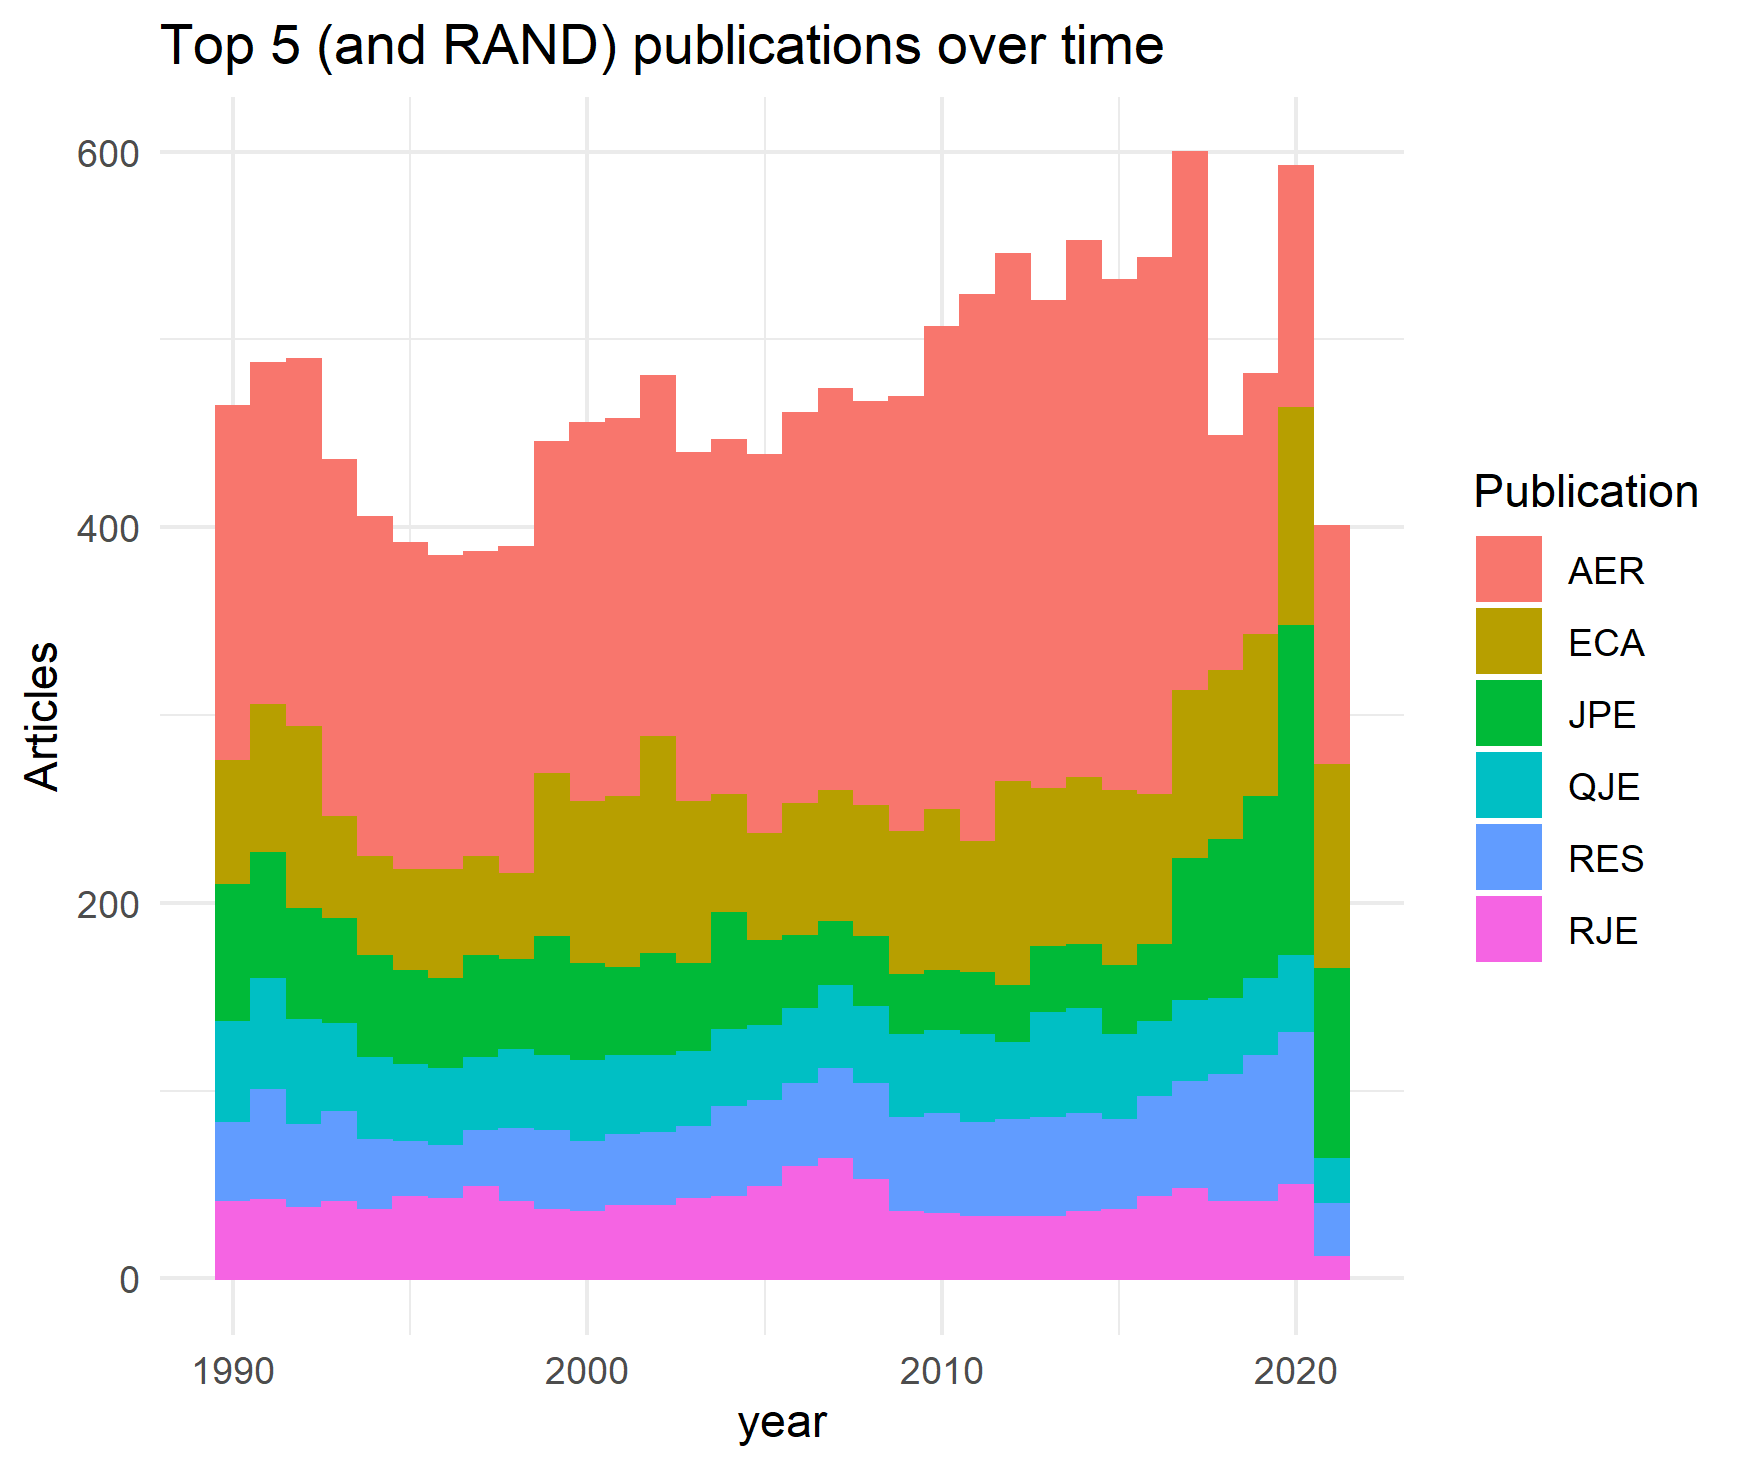
\includegraphics[width=\textwidth]{top_5_over_time_col.png}
        \caption{By count}
    \end{subfigure}
    \hfill
    \begin{subfigure}[h]{0.49\textwidth}
        \centering
        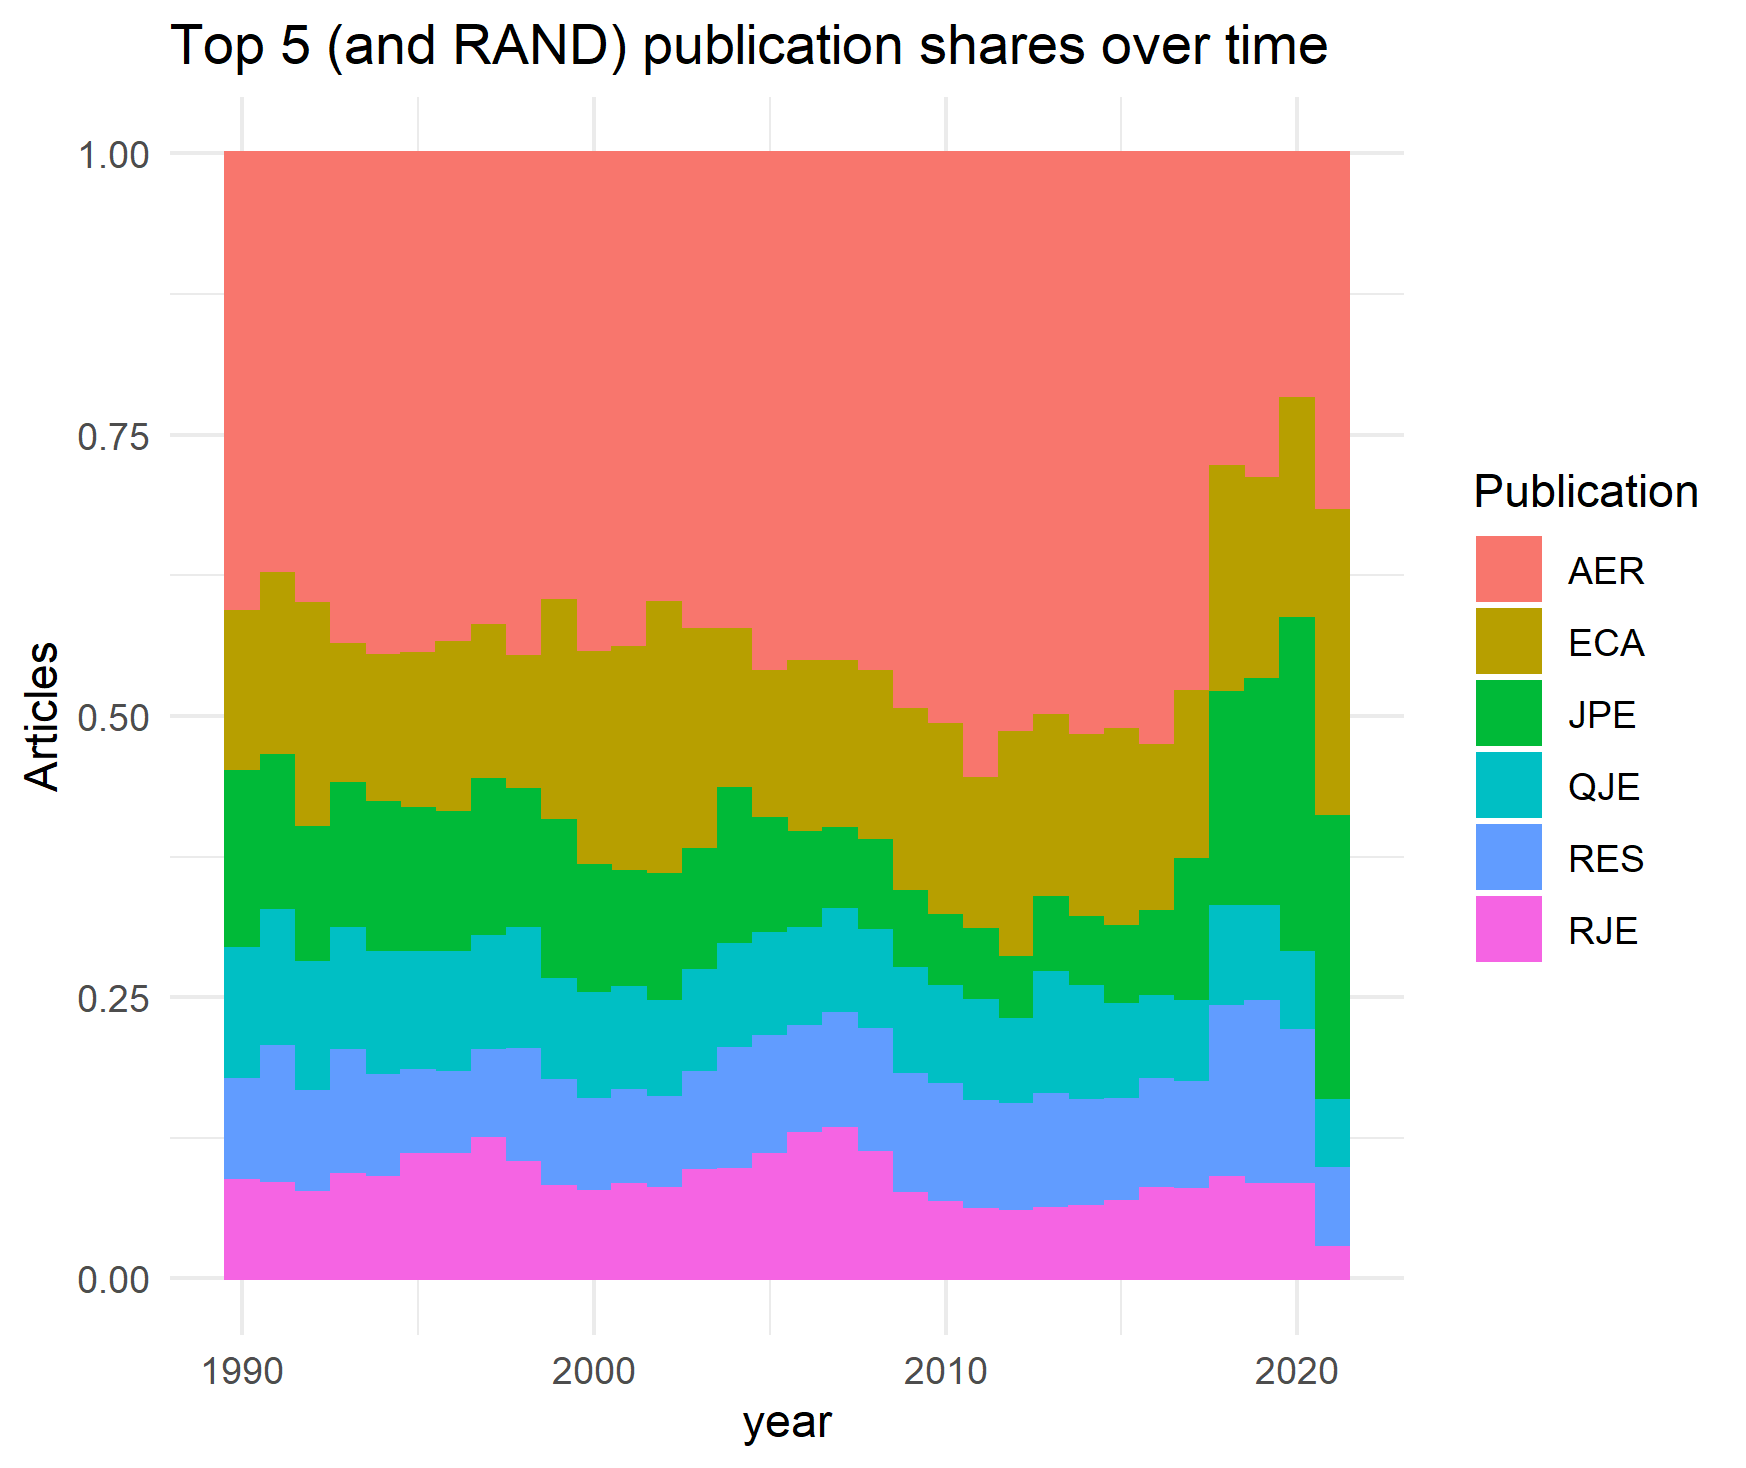
\includegraphics[width=\textwidth]{top_5_over_time_col_shares.png}
        \caption{By share}
    \end{subfigure}
    \begin{subfigure}[h]{\textwidth}
        \centering
        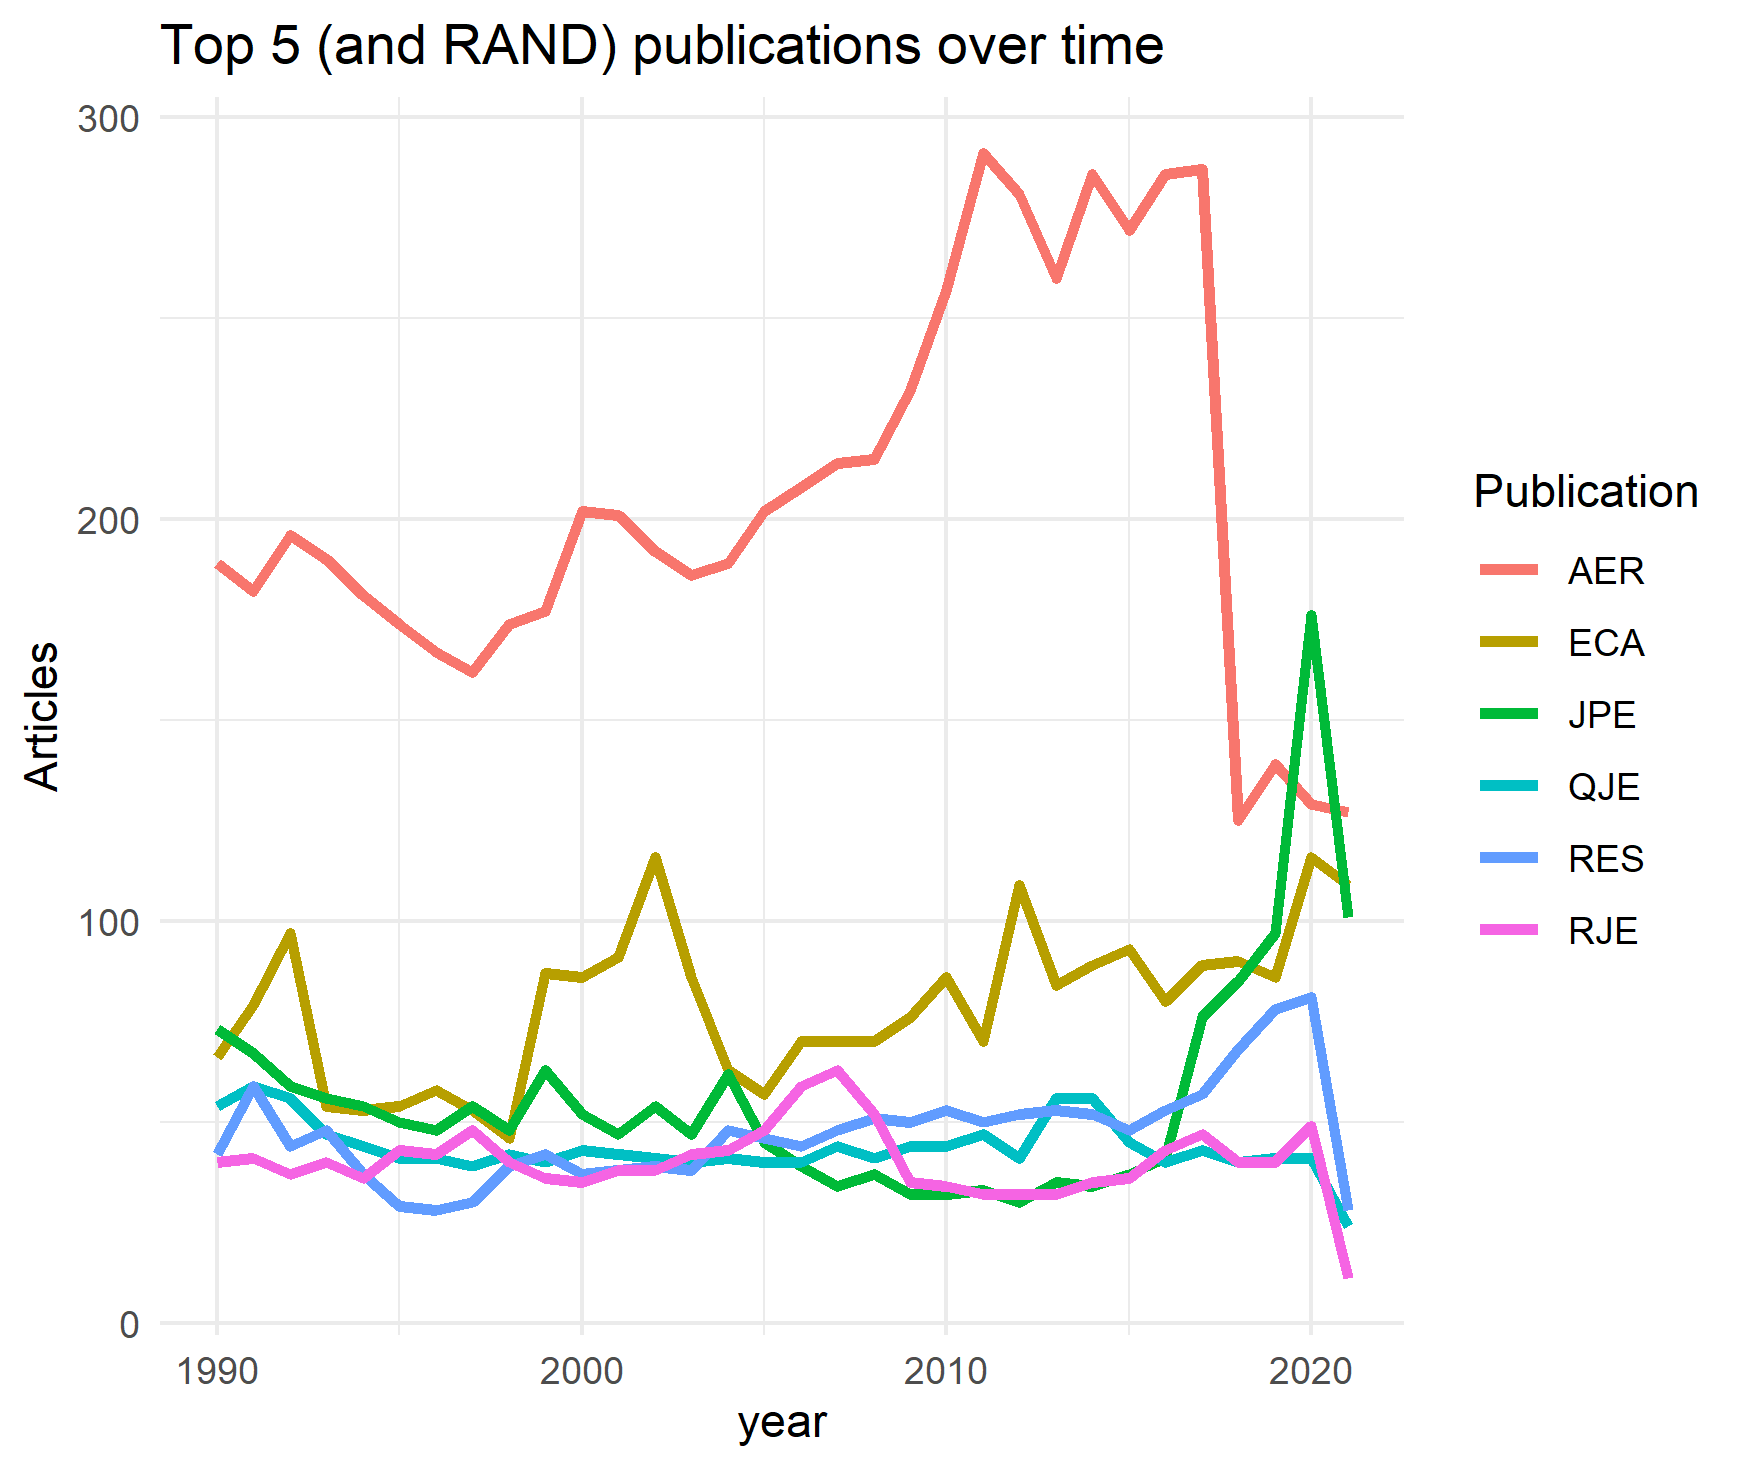
\includegraphics[width=0.5\textwidth]{top5_over_time.png}
        \caption{By count}
    \end{subfigure}
\end{figure}

Though there has been some fluctuation over time, the Top 5 (and RAND) collectively published between 390 and 600 articles per year, with an average of 471 publications per year between 1990 and 2021.\footnote{Note that 2021 may bias this average downwards as not all articles may have yet been indexed by EconLit. Hereafter, we trim all data data to consider only the period from 1991 to 2020.} See Appendix A for a full table of annual publication figures.




\section{The Role of Industrial Organization}
We then consider how Industrial Organization (IO) papers have featured in the Top 5 and RAND over time. We consider a paper to be an ``IO'' publication if the article's associated Journal of Economic Literature (JEL) codes contains \textit{at least} one code that begins with ``L,'' hereafter regularly referred to as LXX. (JEL codes since 1990 have been a letter followed by two numbers, each indicating a greater degree of topic-specificity.) There are other JEL codes which could ostensibly be considered IO-related. These include K21 (Antitrust law), D4 (Market structure, pricing, and design), O3 (Innovation; research and development; technological change; intellectual property rights), and G34 (Mergers; acquisitions; restructuring; corporate governance). However, these are omitted at first to make comparisons (see subsection INSERT NUMBER HERE) across various topics/groups easier. For figures representing a broader definition of IO see appendix INSERT LETTER HERE.\\
\begin{figure}[h]
    \caption{The share of Top 5 (and RAND) articles that are IO related (LXX)}
    \begin{subfigure}[h]{0.49\textwidth}
        \centering
        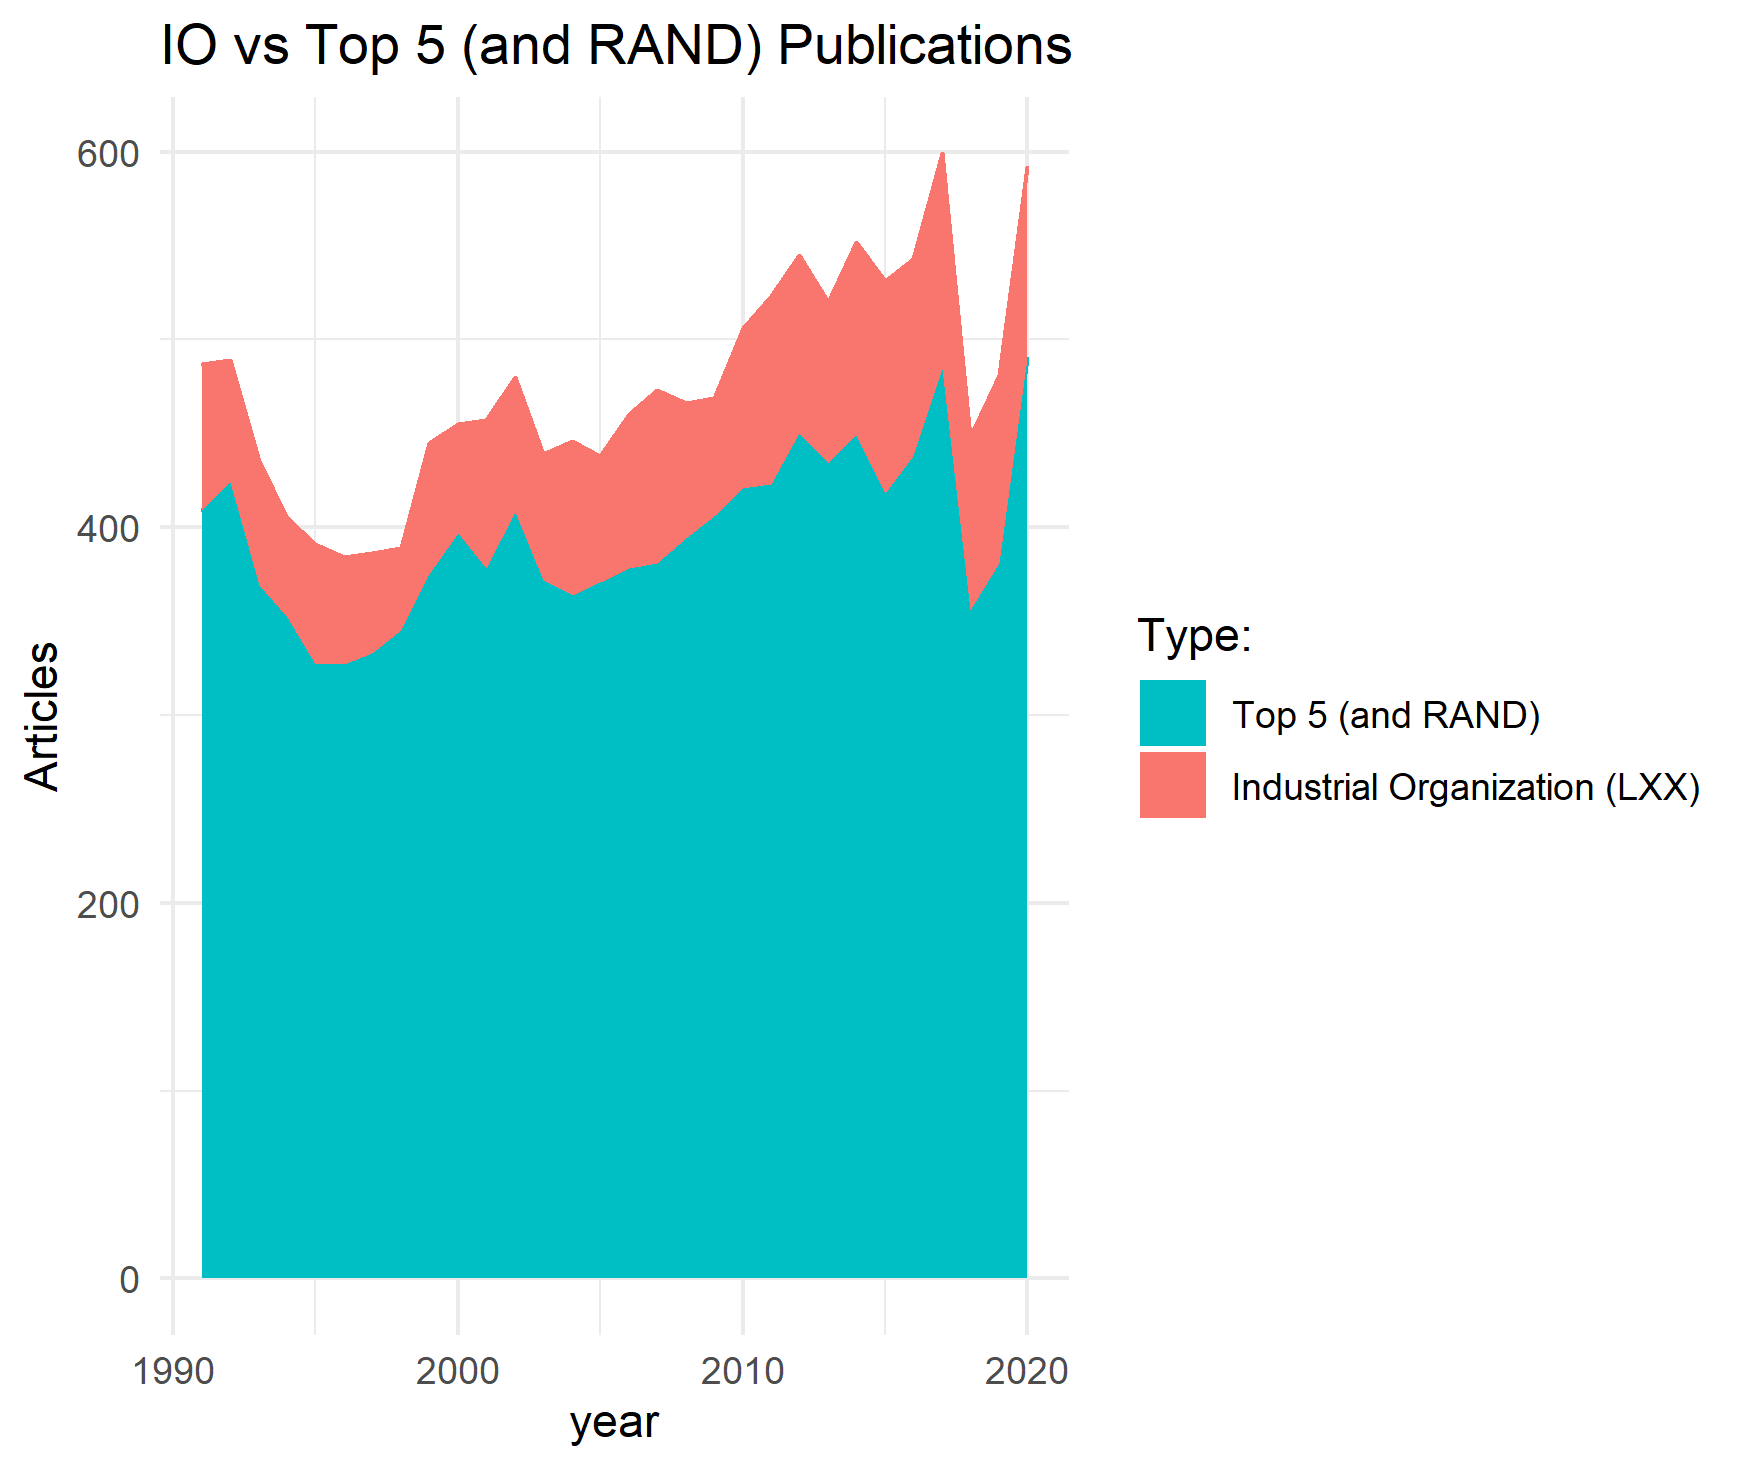
\includegraphics[width=\textwidth]{LXX-code-share-area.png}
        \caption{By count}
    \end{subfigure}
    \hfill
    \begin{subfigure}[h]{0.49\textwidth}
        \centering
        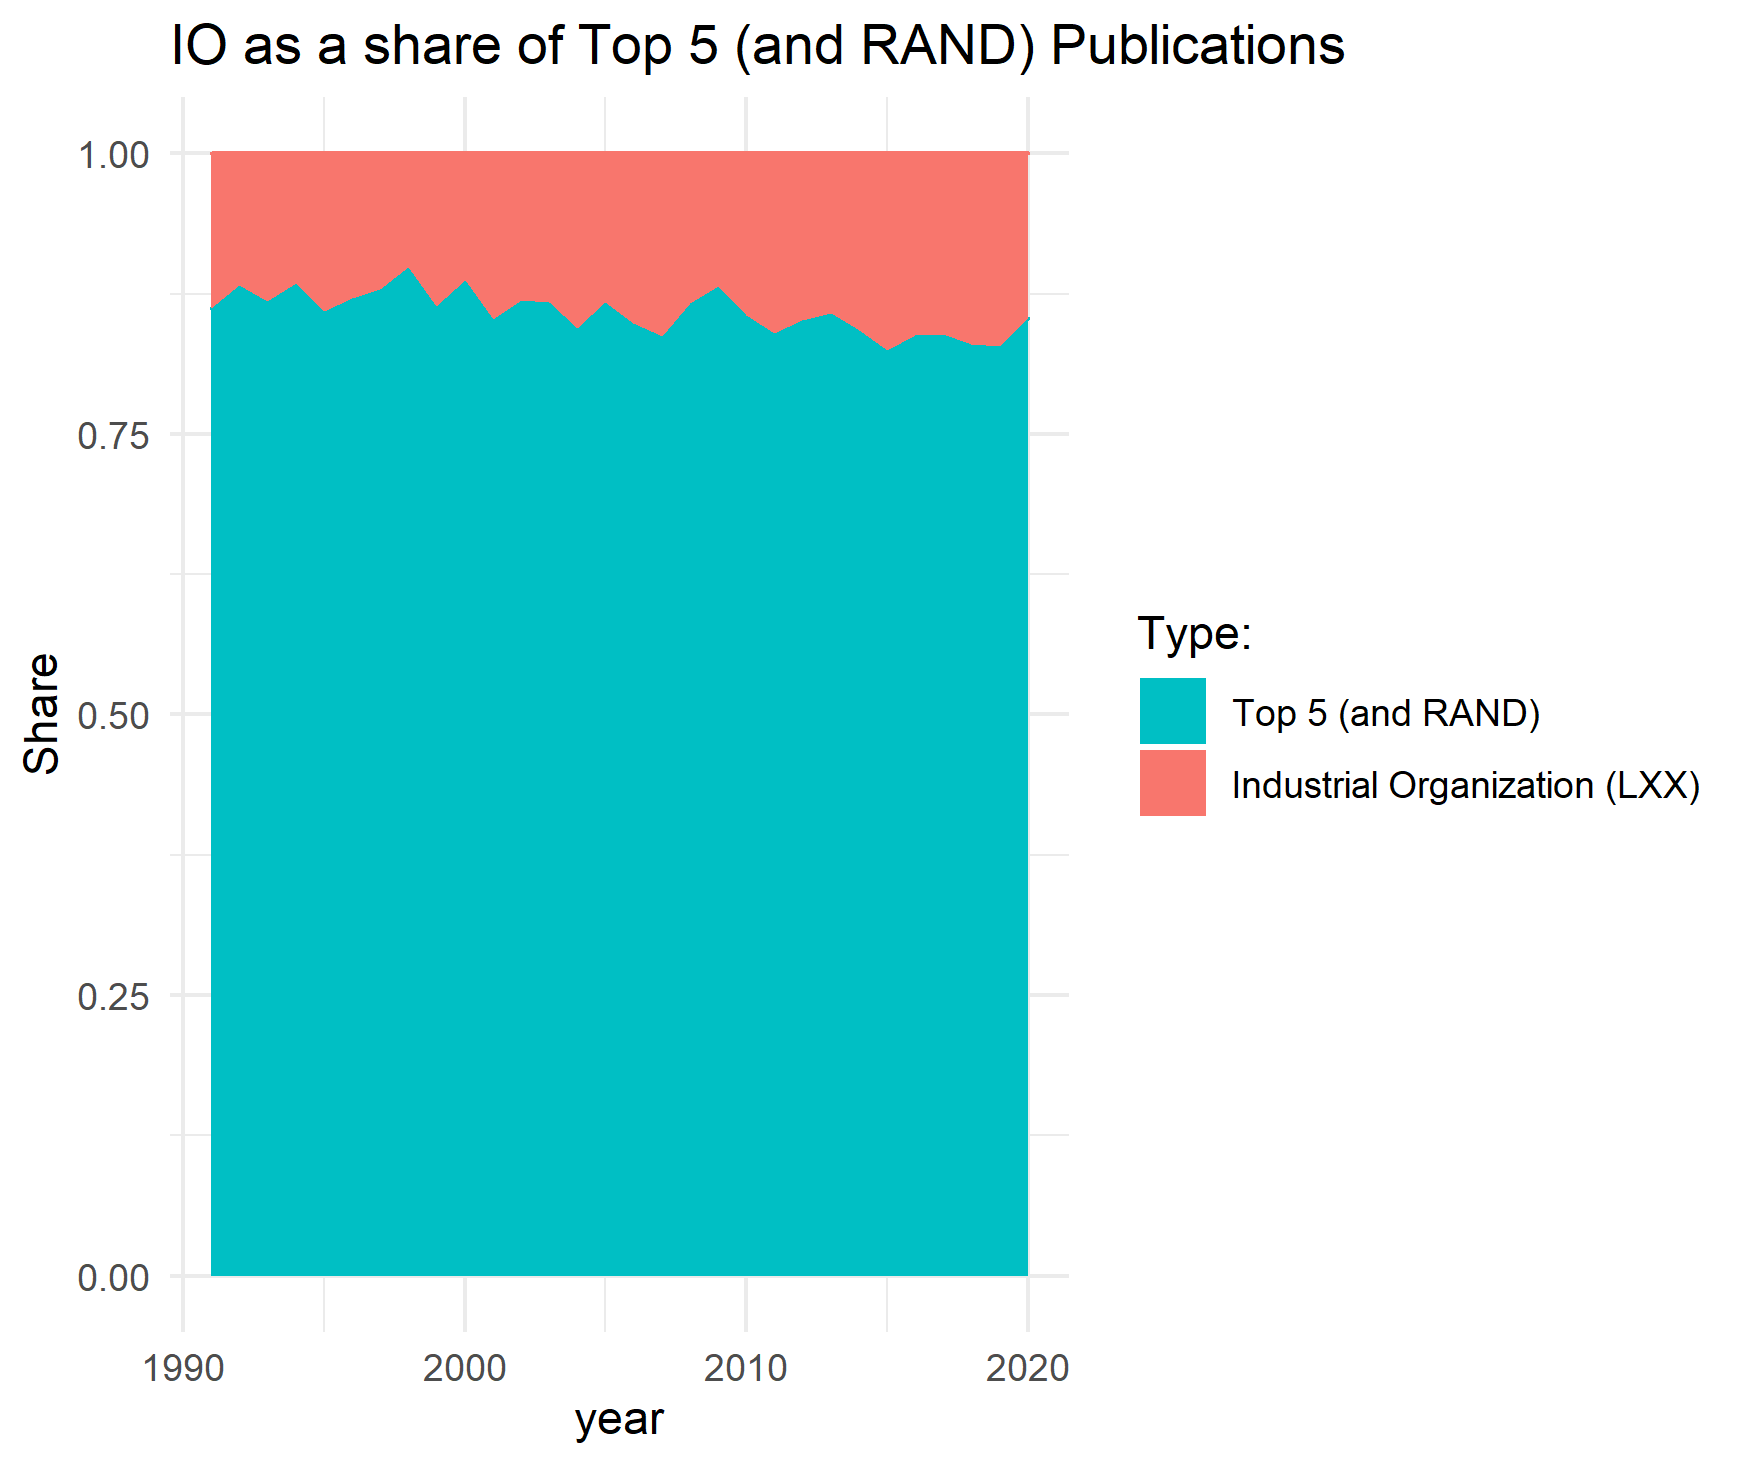
\includegraphics[width=\textwidth]{LXX-code-share-area-normalized.png}
        \caption*{By share}
    \end{subfigure}
\end{figure}

During the the period from 1990 to 2020, IO papers have made up, on average, approximately 16\% of articles published in the Top 5 (and RAND). This share has grown steadily over time, with the greatest share of such articles having been published in 2020 (20.8\%).\footnote{See Appendix INSERT LETTER HERE for a full table of annual IO share figures.} This pattern, however, is not agnostic to journal. That is AER and QJE, publish lots of IO papers relative to, for example, \textit{Econometrica}. Additionally, as a field journal, \textit{RAND} regularly sees almost 40\% its publications mention at least one LXX JEL code.\footnote{For an annual breakdown of by-journal IO shares, please see Appendix INSERT LETTER HERE.}\\

\begin{figure}
    \begin{subfigure}[h]{0.49\textwidth}
        \centering
        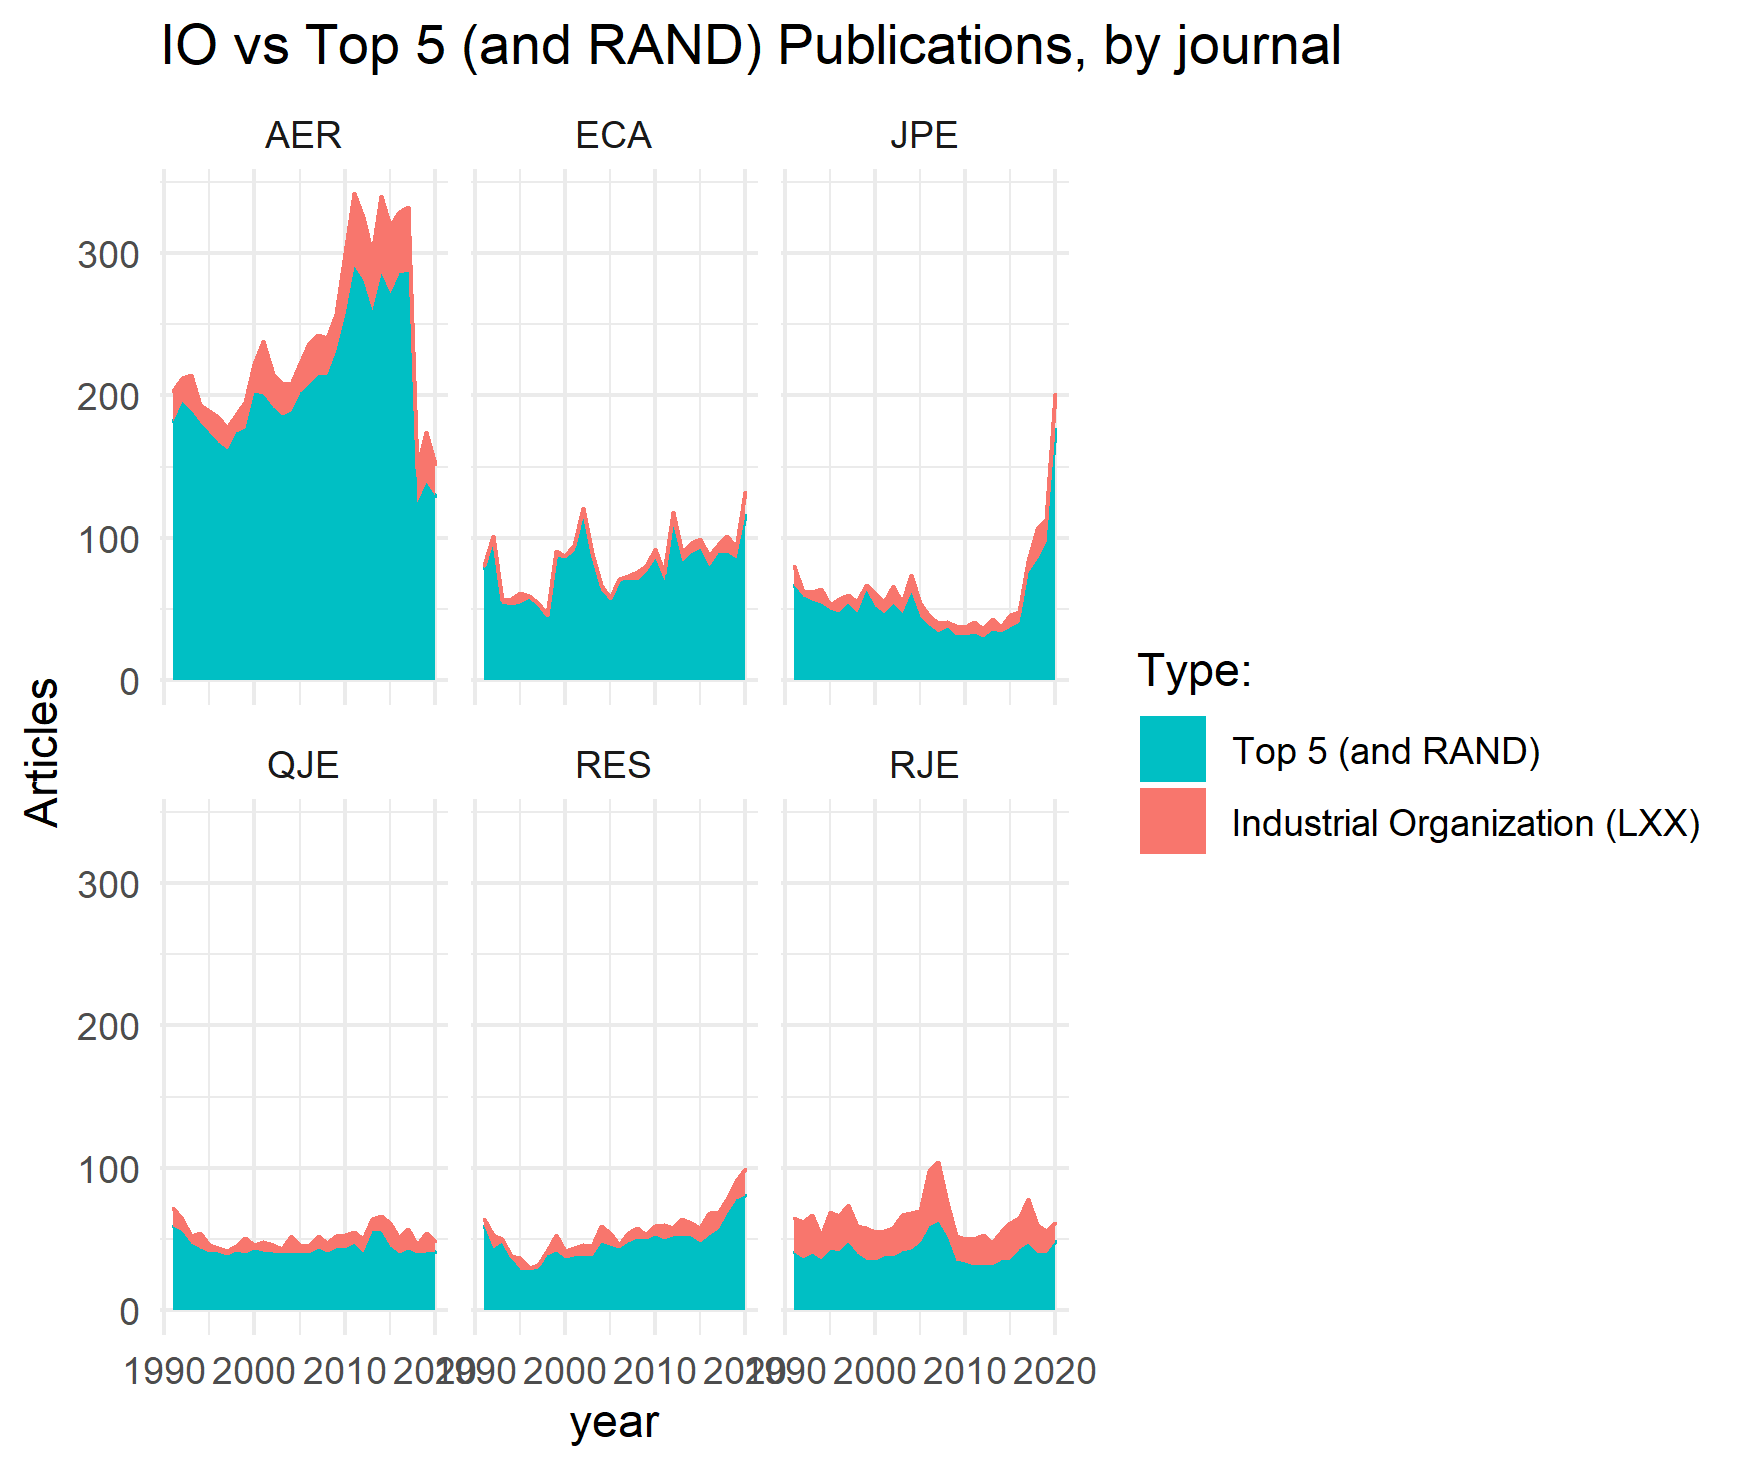
\includegraphics[width=\textwidth]{LXX-code-share-area-by-journal.png}
    \end{subfigure}
    \hfill
    \begin{subfigure}[h]{0.49\textwidth}
        \centering
        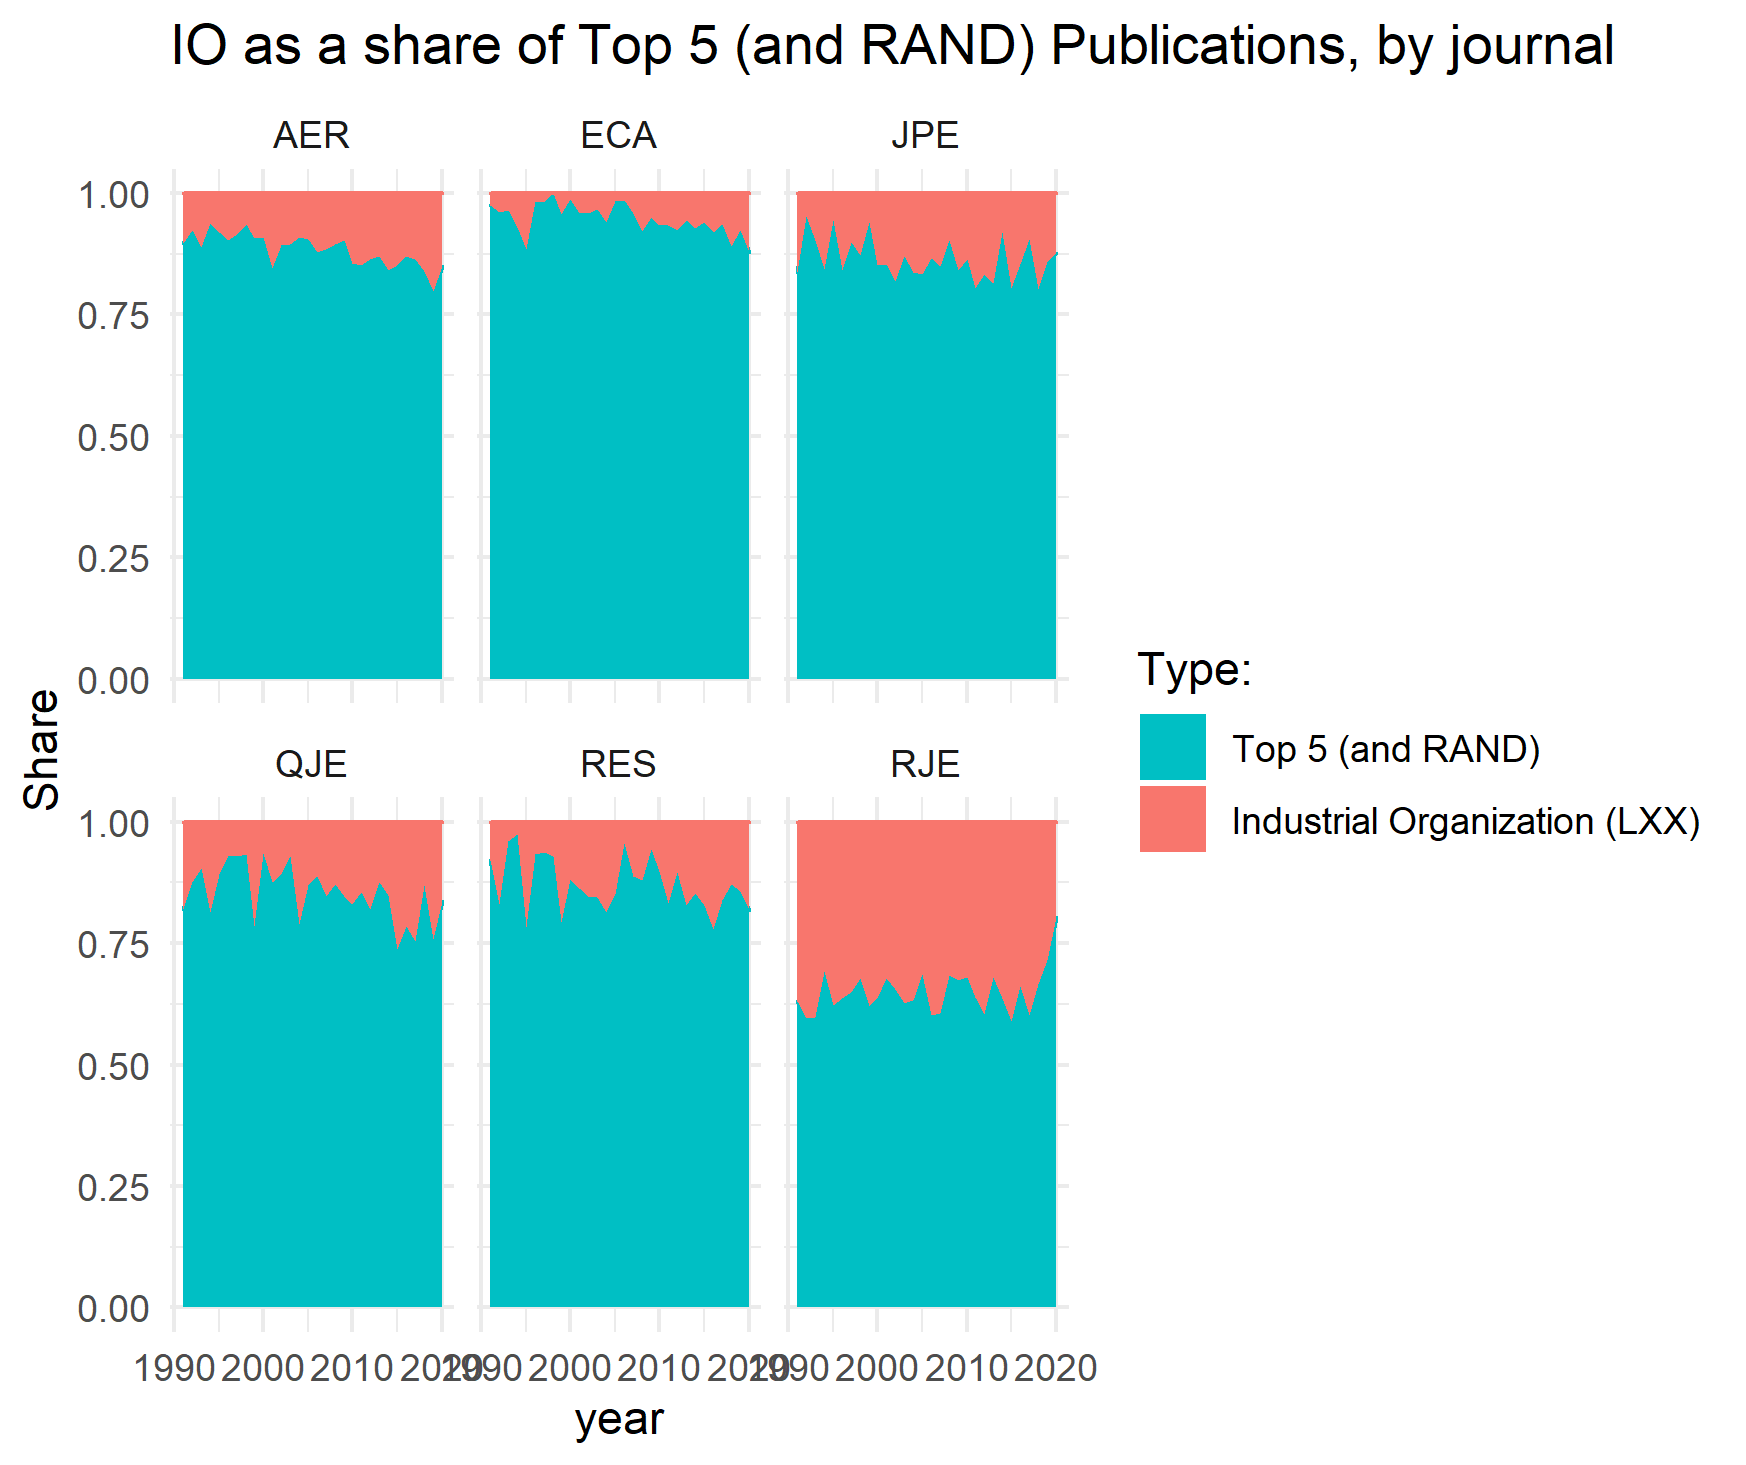
\includegraphics[width=\textwidth]{LXX-code-share-area-normalized-by-journal.png}
    \end{subfigure}
\end{figure}

\newpage

\section{The Role of Anti-Trust}
Even within ``L'' Industrial Organization category, there are 10 classes of JEL codes that refer to topics from ``Market structure, firm strategy and market performance'' (L1) to ``Industry studies: transportation and utilities'' (L9). We are particularly interested in the papers published in the Top 5 (and RAND) that bear at least one L4 code, indicating that the paper pertains to ``Antitrust issues and policies.''

\begin{figure}
    \begin{subfigure}[h]{0.49\textwidth}
        \centering
        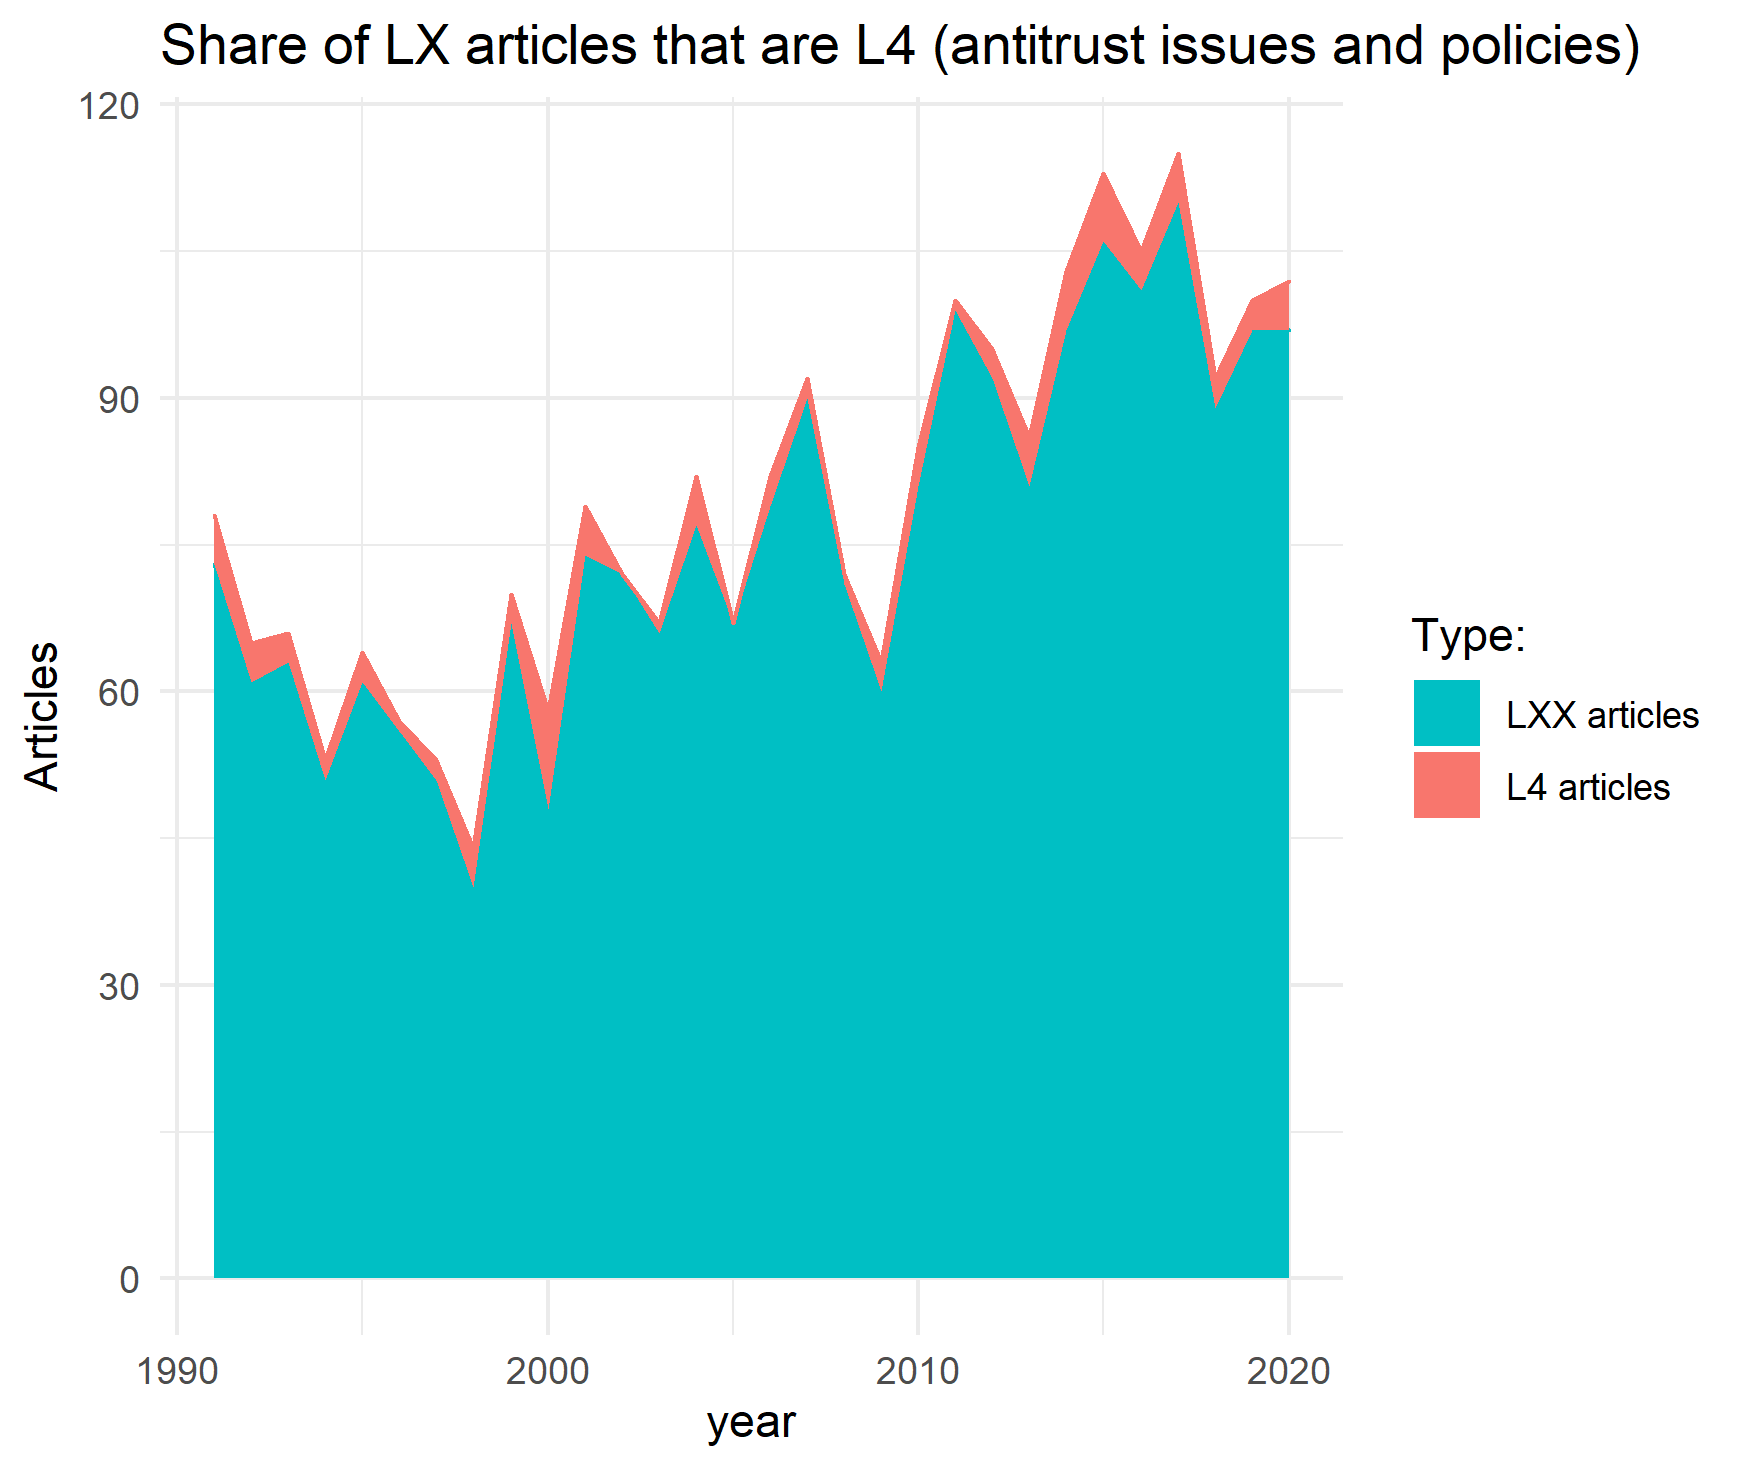
\includegraphics[width=\textwidth]{L4-vs-LXX.png}
    \end{subfigure}
    \hfill
    \begin{subfigure}[h]{0.49\textwidth}
        \centering
        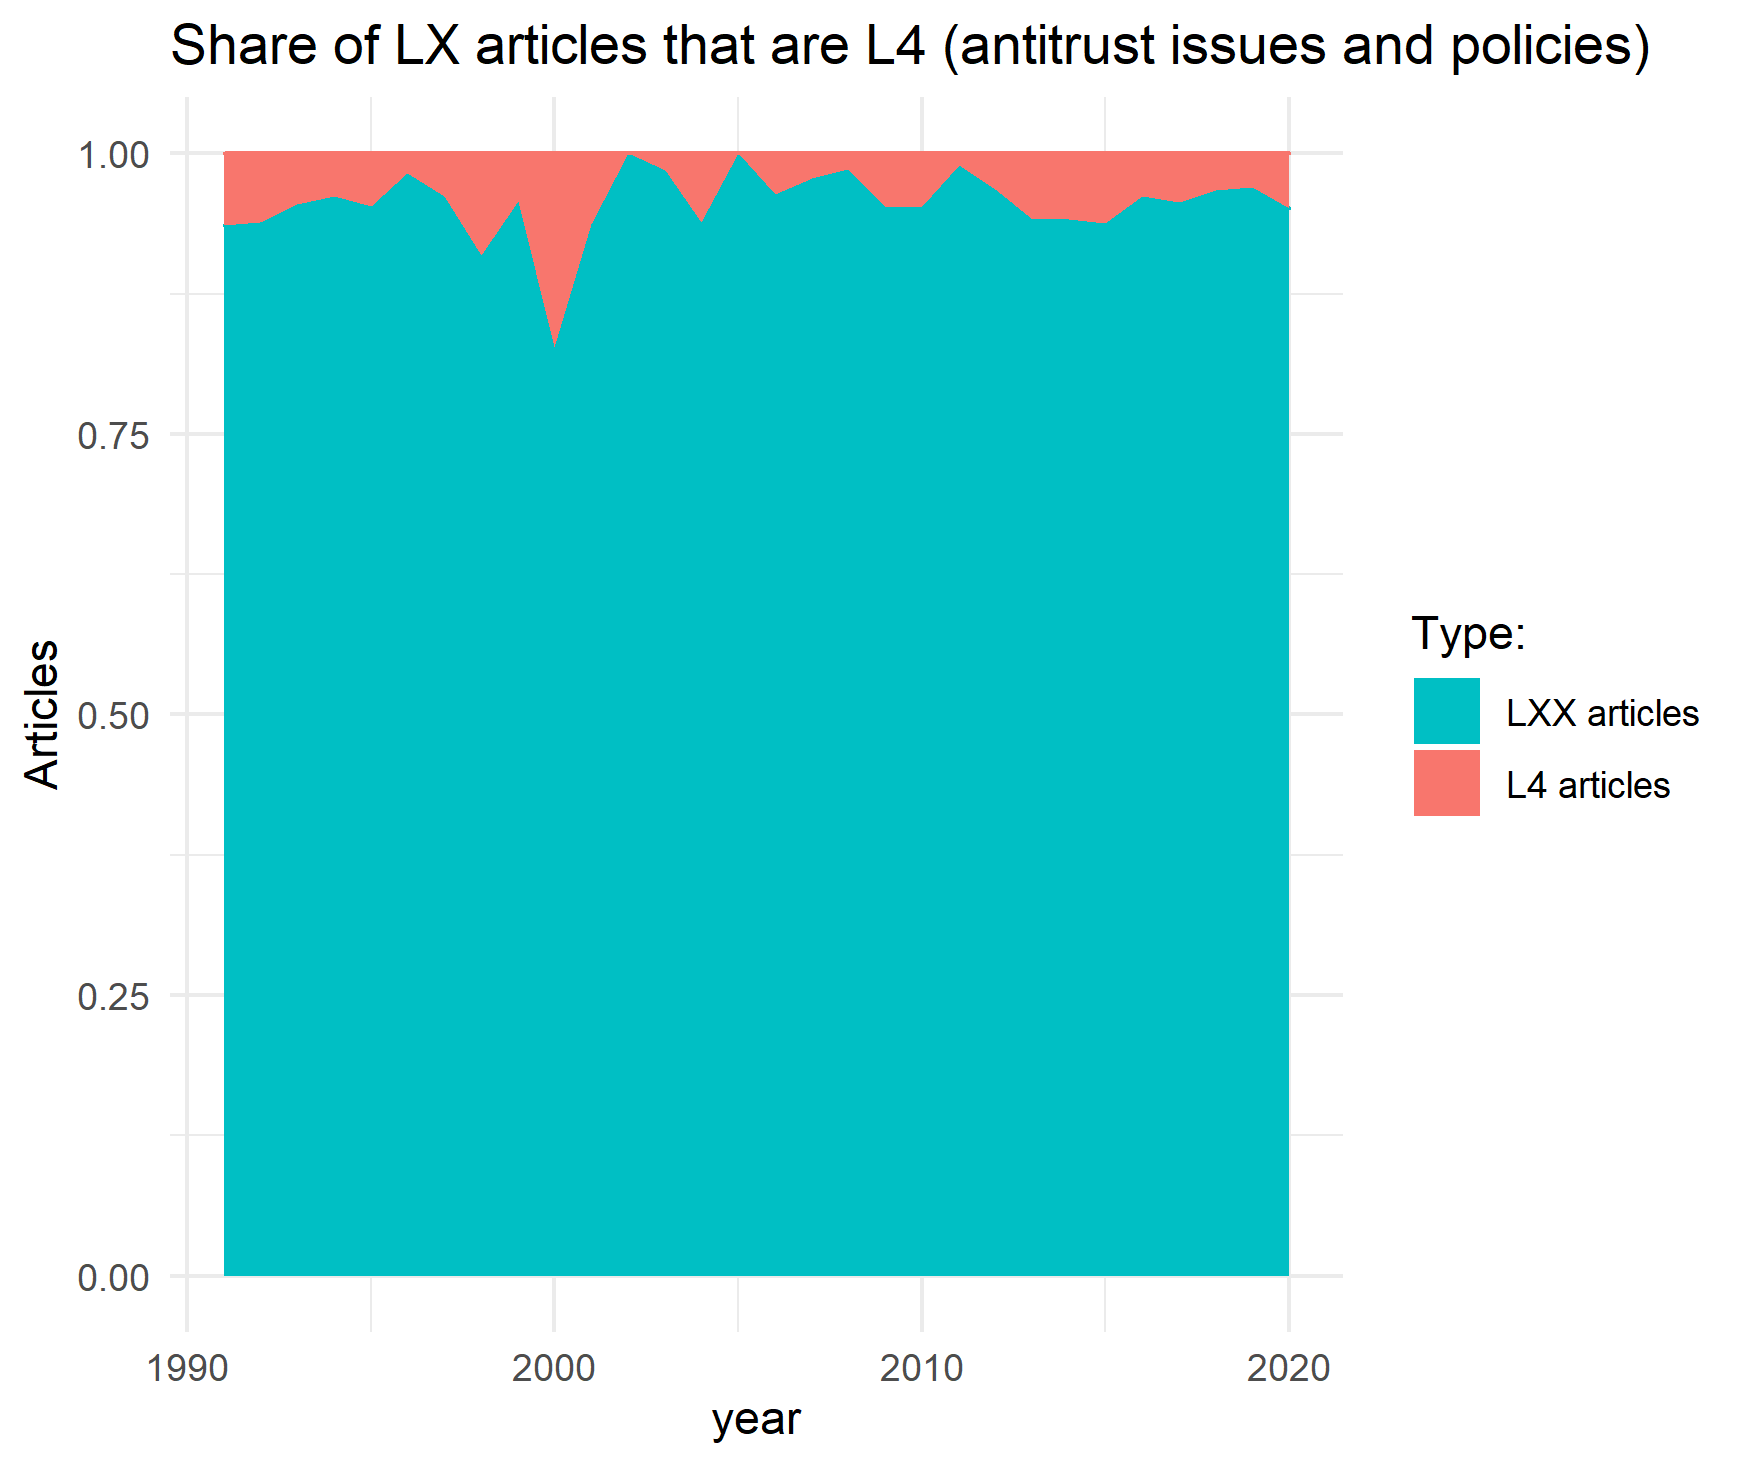
\includegraphics[width=\textwidth]{L4-vs-LXX-normalized.png}
    \end{subfigure}
\end{figure}


\begin{figure}
    \begin{subfigure}[h]{0.49\textwidth}
        \centering
        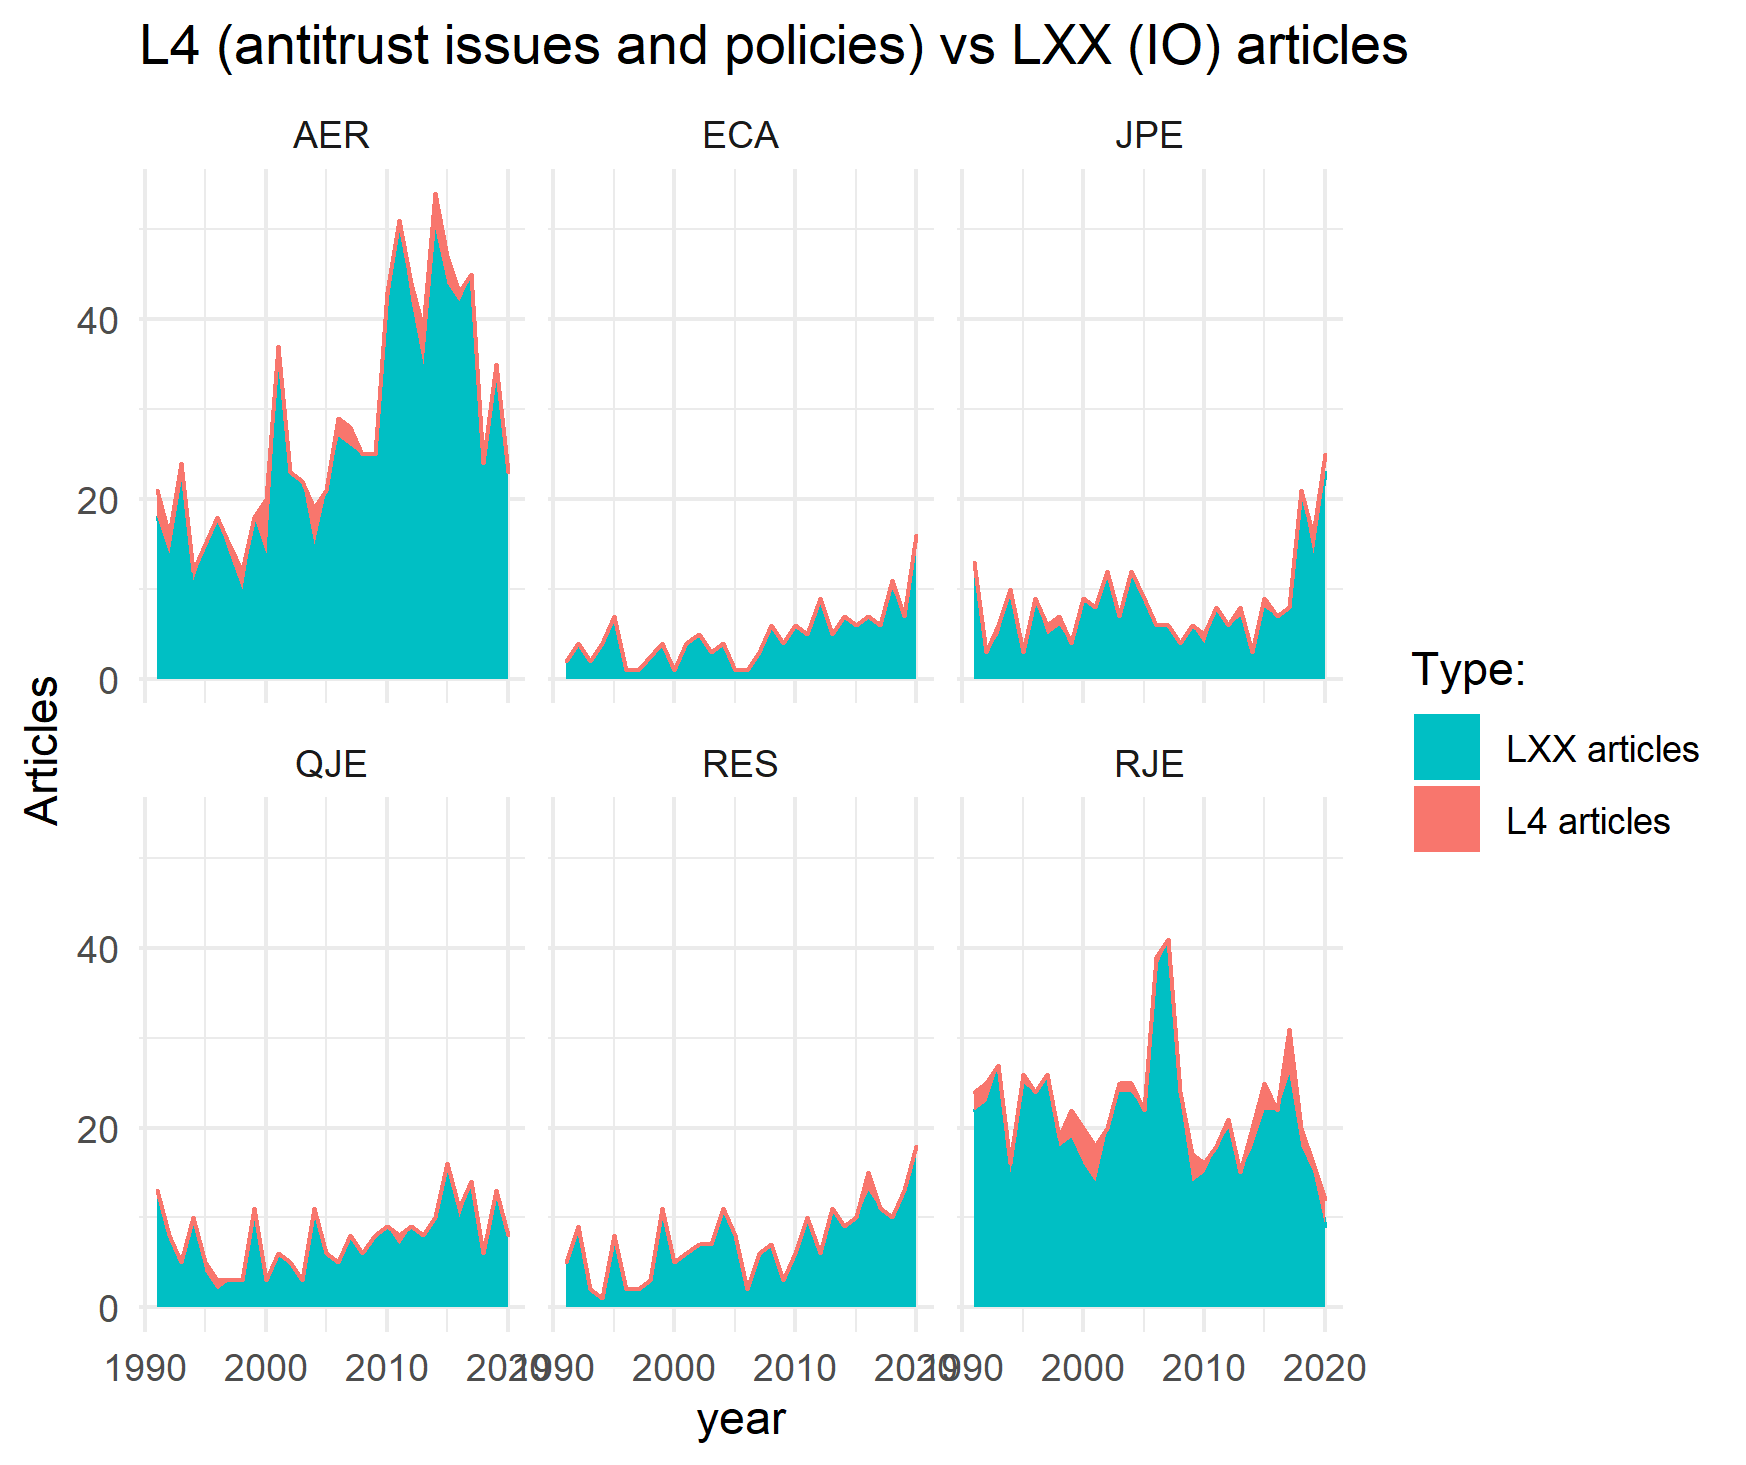
\includegraphics[width=\textwidth]{L4-vs-LXX-by-journal.png}
    \end{subfigure}
    \hfill
    \begin{subfigure}[h]{0.49\textwidth}
        \centering
        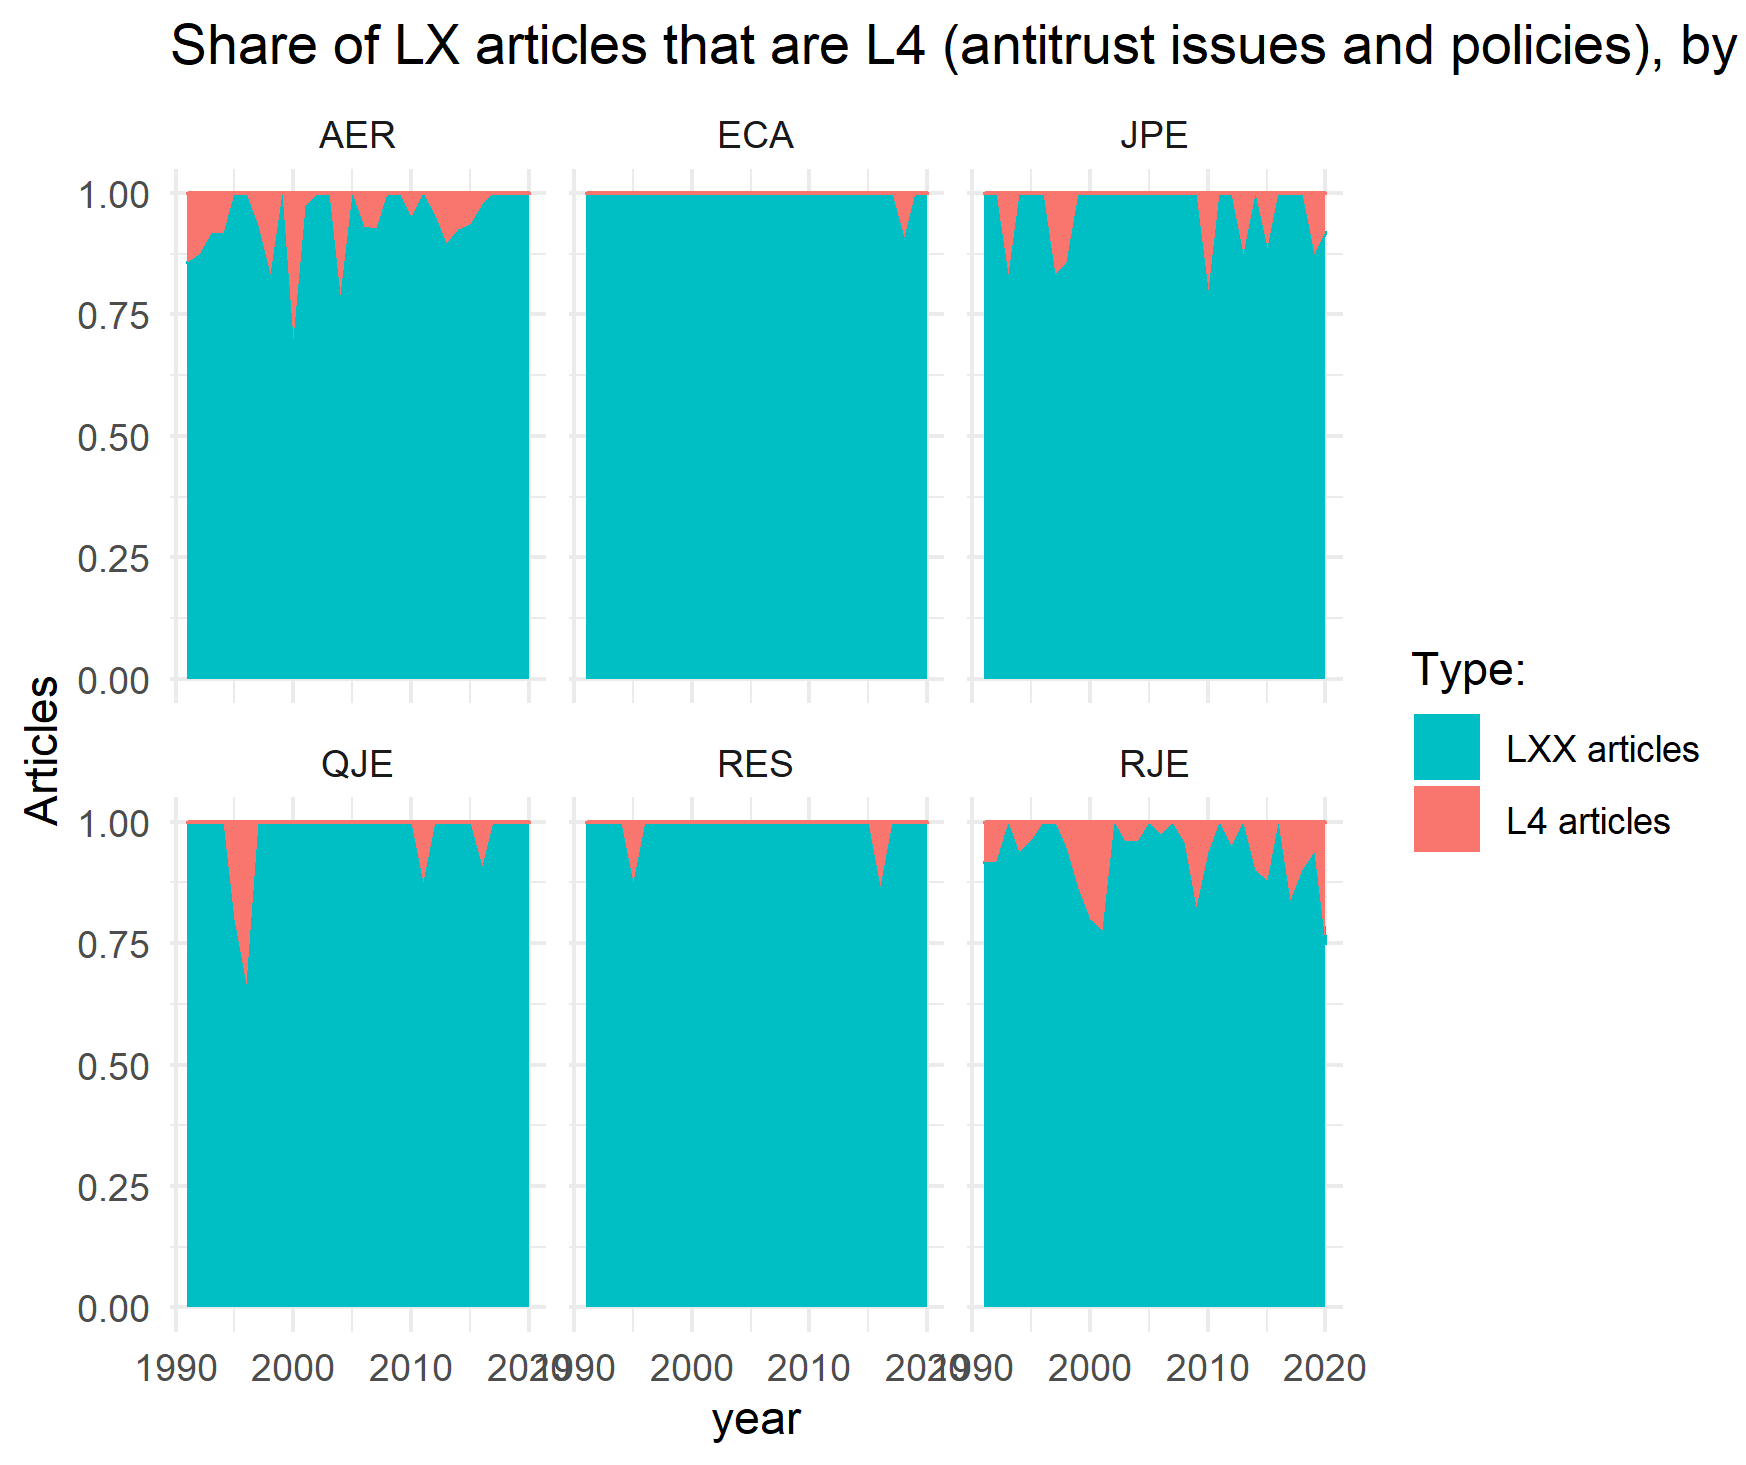
\includegraphics[width=\textwidth]{L4-vs-LXX-normalized-by_journal.png}
    \end{subfigure}
\end{figure}

\subsection{Anti-Trust relative to Wages}

\begin{figure}
    \begin{subfigure}[h]{0.49\textwidth}
        \centering
        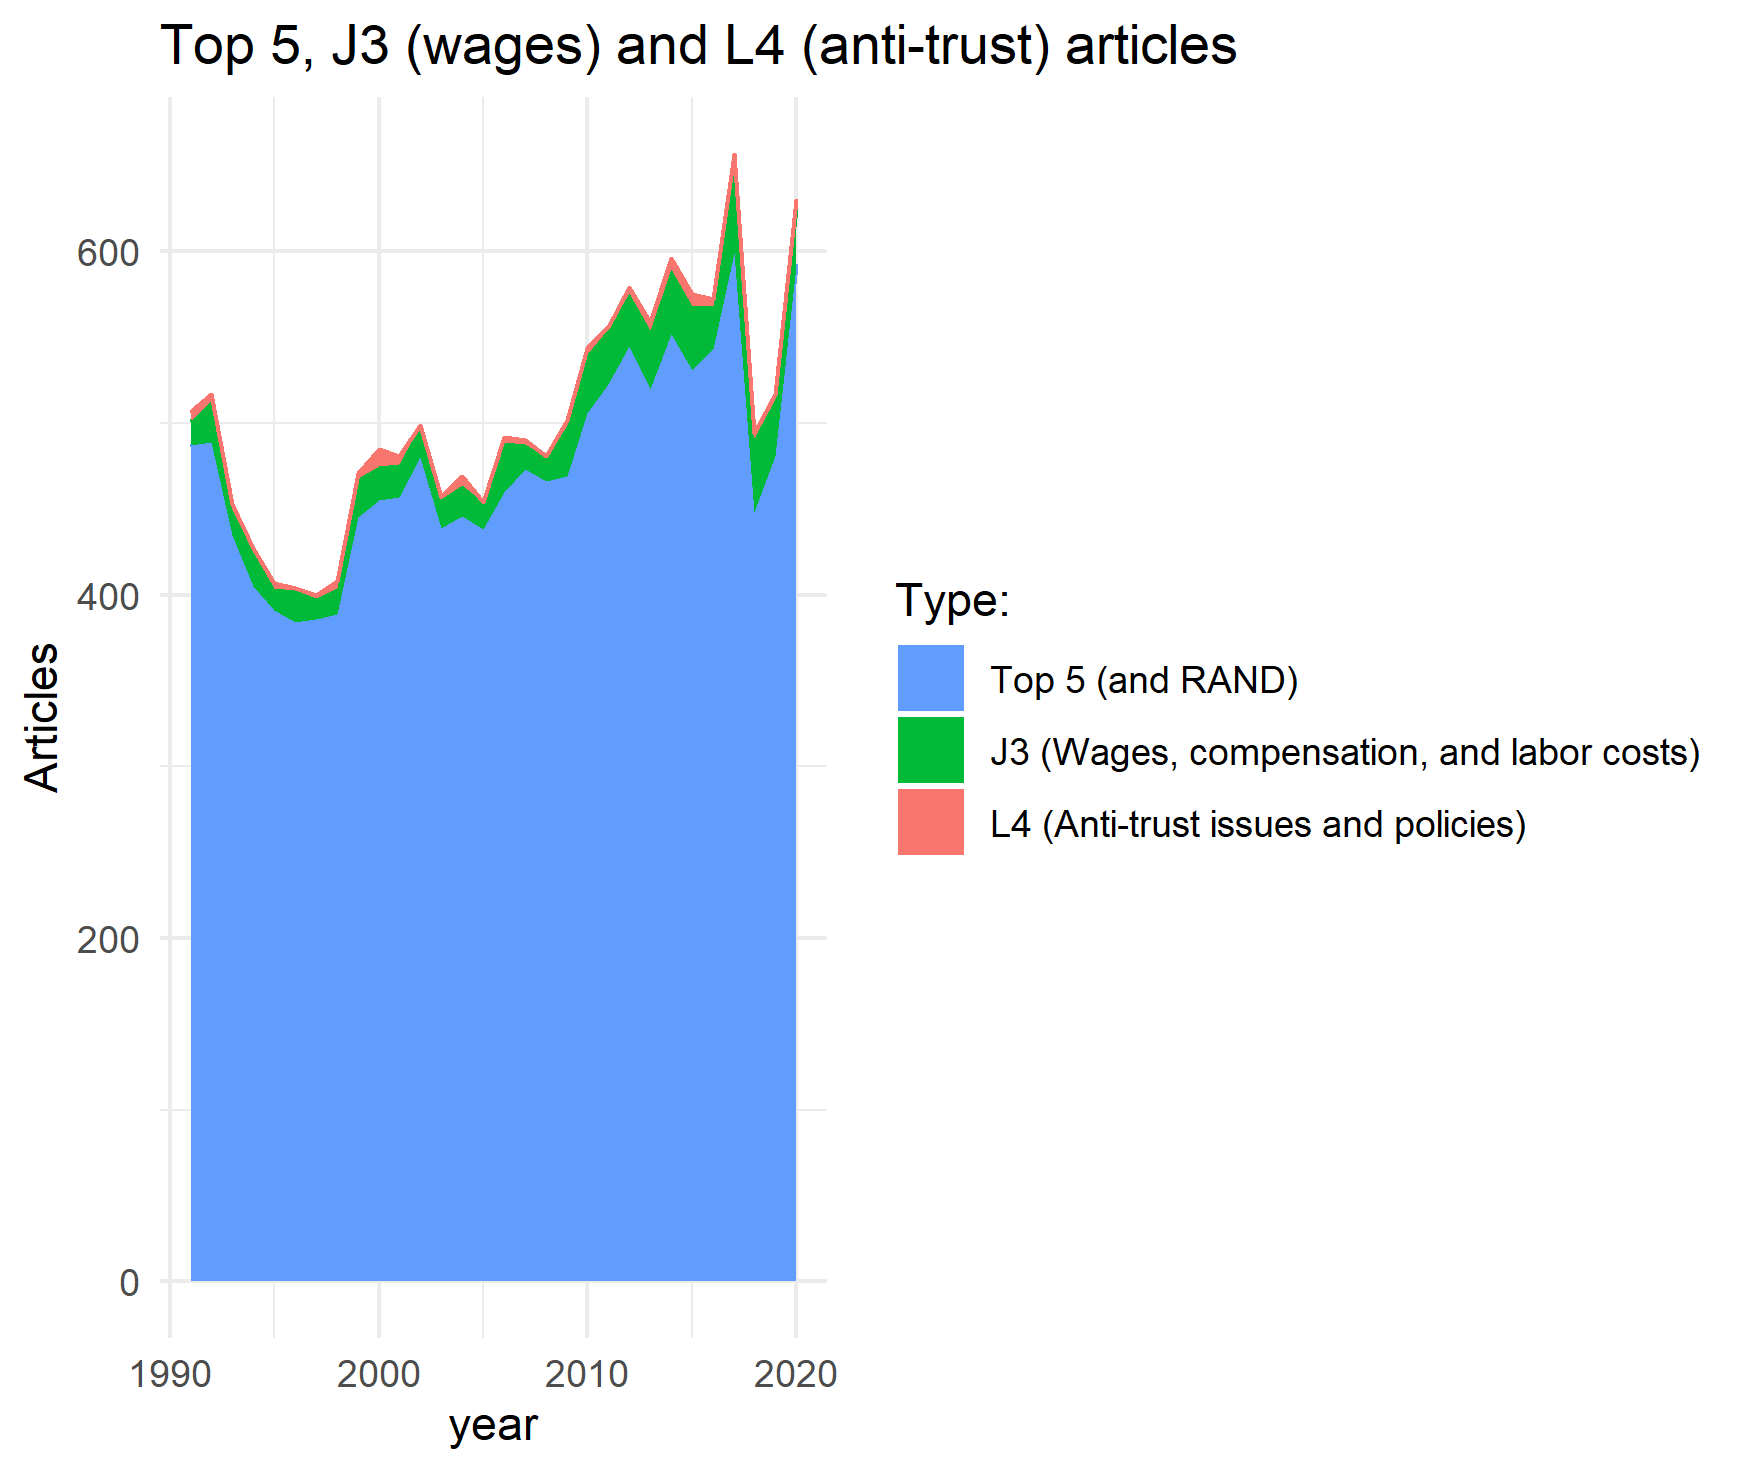
\includegraphics[width=\textwidth]{j3-l4-top5.png}
    \end{subfigure}
    \hfill
    \begin{subfigure}[h]{0.49\textwidth}
        \centering
        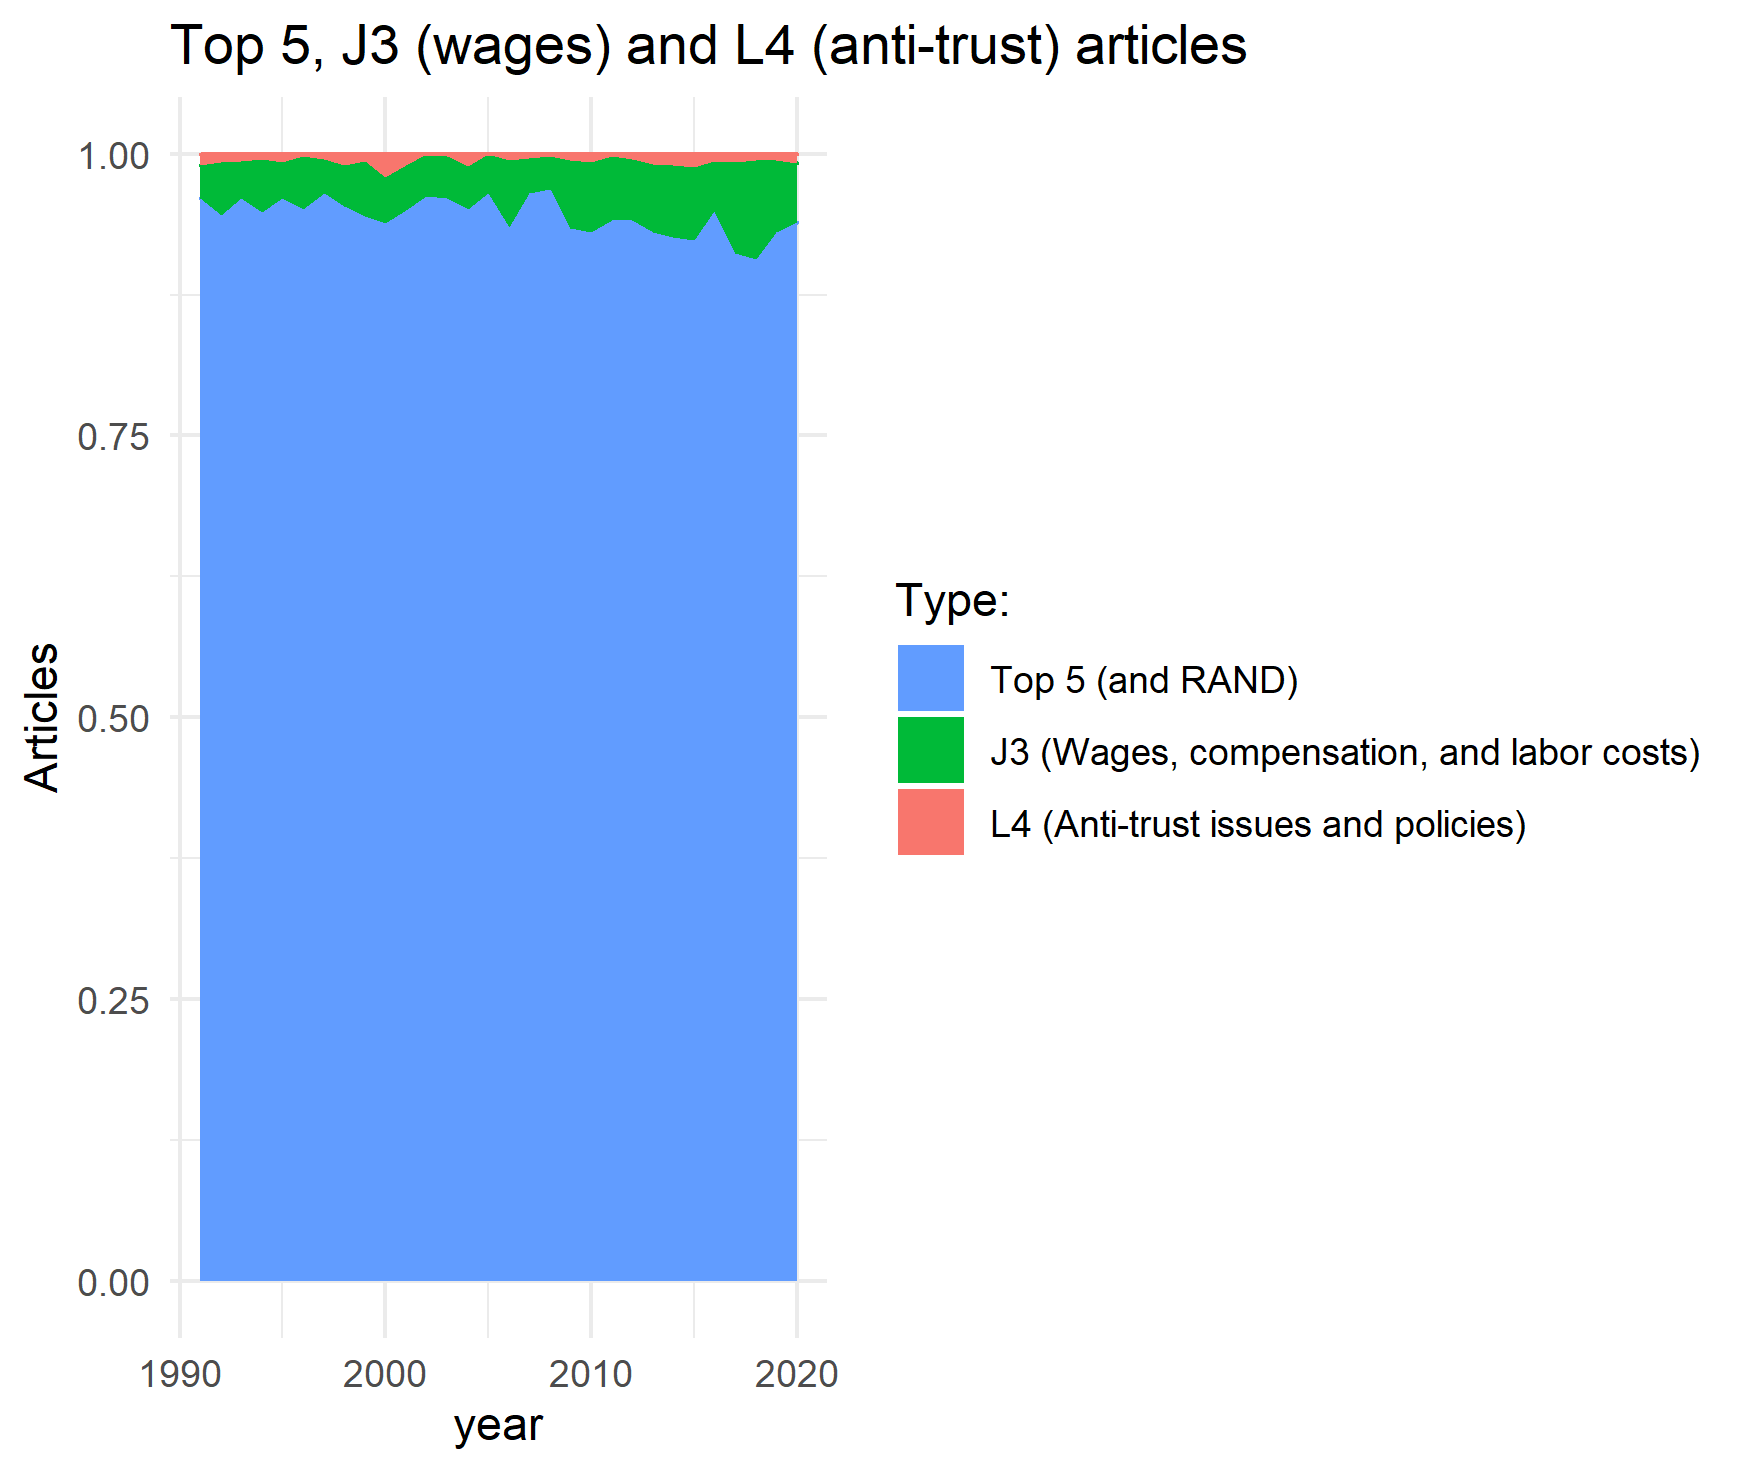
\includegraphics[width=\textwidth]{j3-l4-top5-normalized.png}
    \end{subfigure}
\end{figure}



\appendix
\section{The Production of Academic Articles}

% Table created by stargazer v.5.2.3 by Marek Hlavac, Social Policy Institute. E-mail: marek.hlavac at gmail.com
% Date and time: Thu, Apr 28, 2022 - 3:42:28 PM
\begin{table}[!htbp] \centering 
  \caption{} 
  \label{} 
\footnotesize 
\begin{tabular}{@{\extracolsep{5pt}} cccccccc} 
\\[-1.8ex]\hline 
\hline \\[-1.8ex] 
 & AER & ECA & JPE & QJE & RES & RJE & TOTAL \\ 
\hline \\[-1.8ex] 
1990 & $189$ & $66$ & $73$ & $54$ & $42$ & $40$ & $464$ \\ 
1991 & $182$ & $79$ & $67$ & $59$ & $59$ & $41$ & $487$ \\ 
1992 & $196$ & $97$ & $59$ & $56$ & $44$ & $37$ & $489$ \\ 
1993 & $190$ & $54$ & $56$ & $47$ & $48$ & $40$ & $435$ \\ 
1994 & $181$ & $53$ & $54$ & $44$ & $37$ & $36$ & $405$ \\ 
1995 & $174$ & $54$ & $50$ & $41$ & $29$ & $43$ & $391$ \\ 
1996 & $167$ & $58$ & $48$ & $41$ & $28$ & $42$ & $384$ \\ 
1997 & $162$ & $53$ & $54$ & $39$ & $30$ & $48$ & $386$ \\ 
1998 & $174$ & $46$ & $48$ & $42$ & $39$ & $40$ & $389$ \\ 
1999 & $177$ & $87$ & $63$ & $40$ & $42$ & $36$ & $445$ \\ 
2000 & $202$ & $86$ & $52$ & $43$ & $37$ & $35$ & $455$ \\ 
2001 & $201$ & $91$ & $47$ & $42$ & $38$ & $38$ & $457$ \\ 
2002 & $192$ & $116$ & $54$ & $41$ & $39$ & $38$ & $480$ \\ 
2003 & $186$ & $86$ & $47$ & $40$ & $38$ & $42$ & $439$ \\ 
2004 & $189$ & $63$ & $62$ & $41$ & $48$ & $43$ & $446$ \\ 
2005 & $202$ & $57$ & $45$ & $40$ & $46$ & $48$ & $438$ \\ 
2006 & $208$ & $70$ & $39$ & $40$ & $44$ & $59$ & $460$ \\ 
2007 & $214$ & $70$ & $34$ & $44$ & $48$ & $63$ & $473$ \\ 
2008 & $215$ & $70$ & $37$ & $41$ & $51$ & $52$ & $466$ \\ 
2009 & $232$ & $76$ & $32$ & $44$ & $50$ & $35$ & $469$ \\ 
2010 & $257$ & $86$ & $32$ & $44$ & $53$ & $34$ & $506$ \\ 
2011 & $291$ & $70$ & $33$ & $47$ & $50$ & $32$ & $523$ \\ 
2012 & $281$ & $109$ & $30$ & $41$ & $52$ & $32$ & $545$ \\ 
2013 & $260$ & $84$ & $35$ & $56$ & $53$ & $32$ & $520$ \\ 
2014 & $286$ & $89$ & $34$ & $56$ & $52$ & $35$ & $552$ \\ 
2015 & $272$ & $93$ & $37$ & $45$ & $48$ & $36$ & $531$ \\ 
2016 & $286$ & $80$ & $41$ & $40$ & $53$ & $43$ & $543$ \\ 
2017 & $287$ & $89$ & $76$ & $43$ & $57$ & $47$ & $599$ \\ 
2018 & $125$ & $90$ & $85$ & $40$ & $68$ & $40$ & $448$ \\ 
2019 & $139$ & $86$ & $97$ & $41$ & $78$ & $40$ & $481$ \\ 
2020 & $129$ & $116$ & $176$ & $41$ & $81$ & $49$ & $592$ \\ 
2021 & $127$ & $109$ & $101$ & $24$ & $28$ & $11$ & $400$ \\ 
\hline \\[-1.8ex] 
\end{tabular} 
\end{table} 


\section{The Role of Industrial Organization}

% Table created by stargazer v.5.2.3 by Marek Hlavac, Social Policy Institute. E-mail: marek.hlavac at gmail.com
% Date and time: Fri, Apr 29, 2022 - 1:00:37 PM
\begin{table}[!htbp] \centering 
  \caption{} 
  \label{} 
\footnotesize 
\begin{tabular}{@{\extracolsep{5pt}} cccc} 
\\[-1.8ex]\hline 
\hline \\[-1.8ex] 
 & IO (LXX) & Top 5 (and RAND) & IO Share \\ 
\hline \\[-1.8ex] 
1991 & $78$ & $487$ & 16.0\% \\ 
1992 & $65$ & $489$ & 13.3\% \\ 
1993 & $66$ & $435$ & 15.2\% \\ 
1994 & $53$ & $405$ & 13.1\% \\ 
1995 & $64$ & $391$ & 16.4\% \\ 
1996 & $57$ & $384$ & 14.8\% \\ 
1997 & $53$ & $386$ & 13.7\% \\ 
1998 & $44$ & $389$ & 11.3\% \\ 
1999 & $70$ & $445$ & 15.7\% \\ 
2000 & $58$ & $455$ & 12.7\% \\ 
2001 & $79$ & $457$ & 17.3\% \\ 
2002 & $72$ & $480$ & 15.0\% \\ 
2003 & $67$ & $439$ & 15.3\% \\ 
2004 & $82$ & $446$ & 18.4\% \\ 
2005 & $67$ & $438$ & 15.3\% \\ 
2006 & $82$ & $460$ & 17.8\% \\ 
2007 & $92$ & $473$ & 19.5\% \\ 
2008 & $72$ & $466$ & 15.5\% \\ 
2009 & $63$ & $469$ & 13.4\% \\ 
2010 & $85$ & $506$ & 16.8\% \\ 
2011 & $100$ & $523$ & 19.1\% \\ 
2012 & $95$ & $545$ & 17.4\% \\ 
2013 & $86$ & $520$ & 16.5\% \\ 
2014 & $103$ & $552$ & 18.7\% \\ 
2015 & $113$ & $531$ & 21.3\% \\ 
2016 & $105$ & $543$ & 19.3\% \\ 
2017 & $115$ & $599$ & 19.2\% \\ 
2018 & $92$ & $448$ & 20.5\% \\ 
2019 & $100$ & $481$ & 20.8\% \\ 
2020 & $102$ & $592$ & 17.2\% \\ 
\hline \\[-1.8ex] 
\end{tabular} 
\end{table} 



% Table created by stargazer v.5.2.3 by Marek Hlavac, Social Policy Institute. E-mail: marek.hlavac at gmail.com
% Date and time: Fri, Apr 29, 2022 - 1:32:17 PM
\begin{table}[!htbp] \centering 
  \caption{} 
  \label{} 
\footnotesize 
\begin{tabular}{@{\extracolsep{5pt}} ccccccccccccc} 
\\[-1.8ex]\hline 
\hline \\[-1.8ex] 
 & AER & AER IO Share & ECA & ECA IO Share & JPE & JPE IO Share & QJE & QJE IO Share & RES & RES IO Share & RJE & RJE IO Share \\ 
\hline \\[-1.8ex] 
1991 & $182$ & 11.54\% & $79$ & 2.53\% & $67$ & 19.40\% & $59$ & 22.03\% & $59$ & 8.47\% & $41$ & 58.54\% \\ 
1992 & $196$ & 8.16\% & $97$ & 4.12\% & $59$ & 5.08\% & $56$ & 14.29\% & $44$ & 20.45\% & $37$ & 67.57\% \\ 
1993 & $190$ & 12.63\% & $54$ & 3.70\% & $56$ & 10.71\% & $47$ & 10.64\% & $48$ & 4.17\% & $40$ & 67.50\% \\ 
1994 & $181$ & 6.63\% & $53$ & 7.55\% & $54$ & 18.52\% & $44$ & 22.73\% & $37$ & 2.70\% & $36$ & 44.44\% \\ 
1995 & $174$ & 8.62\% & $54$ & 12.96\% & $50$ & 6.00\% & $41$ & 12.20\% & $29$ & 27.59\% & $43$ & 60.47\% \\ 
1996 & $167$ & 10.78\% & $58$ & 1.72\% & $48$ & 18.75\% & $41$ & 7.32\% & $28$ & 7.14\% & $42$ & 57.14\% \\ 
1997 & $162$ & 9.26\% & $53$ & 1.89\% & $54$ & 11.11\% & $39$ & 7.69\% & $30$ & 6.67\% & $48$ & 54.17\% \\ 
1998 & $174$ & 6.90\% & $46$ & 0.00\% & $48$ & 14.58\% & $42$ & 7.14\% & $39$ & 7.69\% & $40$ & 47.50\% \\ 
1999 & $177$ & 10.17\% & $87$ & 4.60\% & $63$ & 6.35\% & $40$ & 27.50\% & $42$ & 26.19\% & $36$ & 61.11\% \\ 
2000 & $202$ & 9.90\% & $86$ & 1.16\% & $52$ & 17.31\% & $43$ & 6.98\% & $37$ & 13.51\% & $35$ & 57.14\% \\ 
2001 & $201$ & 18.41\% & $91$ & 4.40\% & $47$ & 17.02\% & $42$ & 14.29\% & $38$ & 15.79\% & $38$ & 47.37\% \\ 
2002 & $192$ & 11.98\% & $116$ & 4.31\% & $54$ & 22.22\% & $41$ & 12.20\% & $39$ & 17.95\% & $38$ & 52.63\% \\ 
2003 & $186$ & 11.83\% & $86$ & 3.49\% & $47$ & 14.89\% & $40$ & 7.50\% & $38$ & 18.42\% & $42$ & 59.52\% \\ 
2004 & $189$ & 10.05\% & $63$ & 6.35\% & $62$ & 19.35\% & $41$ & 26.83\% & $48$ & 22.92\% & $43$ & 58.14\% \\ 
2005 & $202$ & 10.40\% & $57$ & 1.75\% & $45$ & 20.00\% & $40$ & 15.00\% & $46$ & 17.39\% & $48$ & 45.83\% \\ 
2006 & $208$ & 13.94\% & $70$ & 1.43\% & $39$ & 15.38\% & $40$ & 12.50\% & $44$ & 4.55\% & $59$ & 66.10\% \\ 
2007 & $214$ & 13.08\% & $70$ & 4.29\% & $34$ & 17.65\% & $44$ & 18.18\% & $48$ & 12.50\% & $63$ & 65.08\% \\ 
2008 & $215$ & 11.63\% & $70$ & 8.57\% & $37$ & 10.81\% & $41$ & 14.63\% & $51$ & 13.73\% & $52$ & 46.15\% \\ 
2009 & $232$ & 10.78\% & $76$ & 5.26\% & $32$ & 18.75\% & $44$ & 18.18\% & $50$ & 6.00\% & $35$ & 48.57\% \\ 
2010 & $257$ & 16.73\% & $86$ & 6.98\% & $32$ & 15.62\% & $44$ & 20.45\% & $53$ & 11.32\% & $34$ & 47.06\% \\ 
2011 & $291$ & 17.53\% & $70$ & 7.14\% & $33$ & 24.24\% & $47$ & 17.02\% & $50$ & 20.00\% & $32$ & 56.25\% \\ 
2012 & $281$ & 15.66\% & $109$ & 8.26\% & $30$ & 20.00\% & $41$ & 21.95\% & $52$ & 11.54\% & $32$ & 65.62\% \\ 
2013 & $260$ & 15.00\% & $84$ & 5.95\% & $35$ & 22.86\% & $56$ & 14.29\% & $53$ & 20.75\% & $32$ & 46.88\% \\ 
2014 & $286$ & 18.88\% & $89$ & 7.87\% & $34$ & 8.82\% & $56$ & 17.86\% & $52$ & 17.31\% & $35$ & 57.14\% \\ 
2015 & $272$ & 17.28\% & $93$ & 6.45\% & $37$ & 24.32\% & $45$ & 35.56\% & $48$ & 20.83\% & $36$ & 69.44\% \\ 
2016 & $286$ & 15.03\% & $80$ & 8.75\% & $41$ & 17.07\% & $40$ & 27.50\% & $53$ & 28.30\% & $43$ & 51.16\% \\ 
2017 & $287$ & 15.68\% & $89$ & 6.74\% & $76$ & 10.53\% & $43$ & 32.56\% & $57$ & 19.30\% & $47$ & 65.96\% \\ 
2018 & $125$ & 19.20\% & $90$ & 12.22\% & $85$ & 24.71\% & $40$ & 15.00\% & $68$ & 14.71\% & $40$ & 50.00\% \\ 
2019 & $139$ & 25.18\% & $86$ & 8.14\% & $97$ & 16.49\% & $41$ & 31.71\% & $78$ & 16.67\% & $40$ & 40.00\% \\ 
2020 & $129$ & 17.83\% & $116$ & 13.79\% & $176$ & 14.20\% & $41$ & 19.51\% & $81$ & 22.22\% & $49$ & 24.49\% \\ 
\hline \\[-1.8ex] 
\end{tabular} 
\end{table} 



\newpage

\begin{table}[h] \centering 
    \caption{} 
    \label{} 
    \begin{adjustbox}{max width=\textwidth}
        \begin{tabular}{@{\extracolsep{5pt}} ccccccccccc} 
            \\[-1.8ex]\hline 
            \hline \\[-1.8ex]
            & \multicolumn{6}{c}{\textit{Abstract contains:}} & \multicolumn{4}{c}{\textit{JEL Code}} \\ 
          \cline{2-7} \cline{8-11} \\
            Publication & Anti Trust & Market Power & Anti Competitive & Monopoly & Merger & Cartel & L & K & L4 & K21 \\ 
            \hline \\[-1.8ex] 
            AER & 11 & 25 & 6 & 52 & 30 & 15 & 869 & 216 & 43 & 24 \\ 
            ECA & 1 & 8 & 1 & 22 & 4 & 3 & 154 & 20 & 1 & 7 \\ 
            JPE & 5 & 16 & 1 & 27 & 7 & 5 & 279 & 78 & 12 & 7 \\ 
            QJE & 1 & 12 & 1 & 25 & 8 & 0 & 239 & 60 & 4 & 0 \\ 
            RES & 2 & 9 & 1 & 52 & 5 & 2 & 228 & 39 & 3 & 1 \\ 
            RJE & 21 & 37 & 13 & 113 & 48 & 16 & 679 & 87 & 43 & 15 \\ 
            TOTAL & 41 & 107 & 23 & 291 & 102 & 41 & 2448 & 500 & 106 & 54 \\ 
            \hline \\[-1.8ex] 
        \end{tabular}    
    \end{adjustbox}
\end{table} 



\end{document}